\section{Sample Path Processing Output}%

	Figure~\ref{fig:sample_planning_problem} shows some screenshots of the
	trajectory generation software developed. In the figure, several views
	of a planning problem in a cluttered environment are shown. As can be
	seen, the problem contains obstacles on the ground, on the sides of the
	workspace, as well as hanging from the top of the workspace. The goal is
	to move the end-effector from the start position shown in the figures to
	the opposite corner of the workspace while avoiding collisions.

	\begin{figure}[hbt]
		\centering
		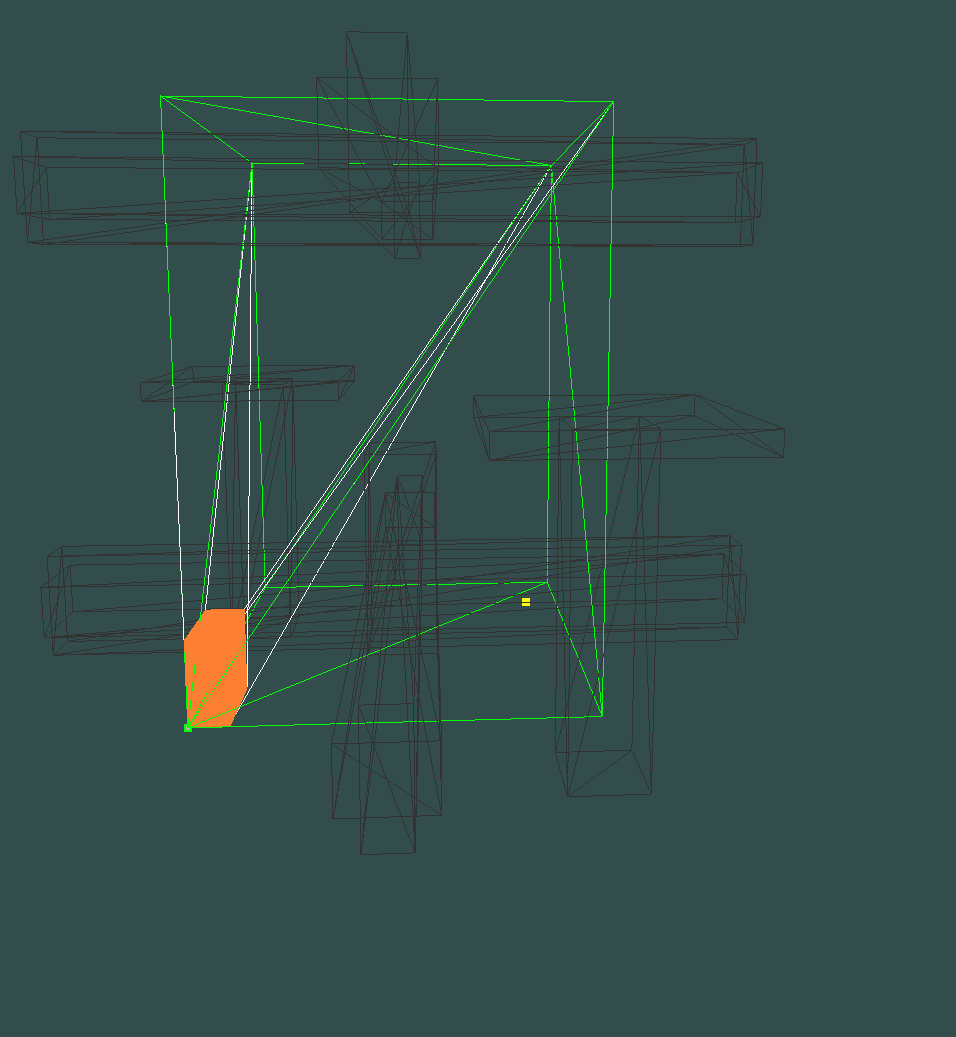
\includegraphics[width=0.3\linewidth]{clutter_front.png}
		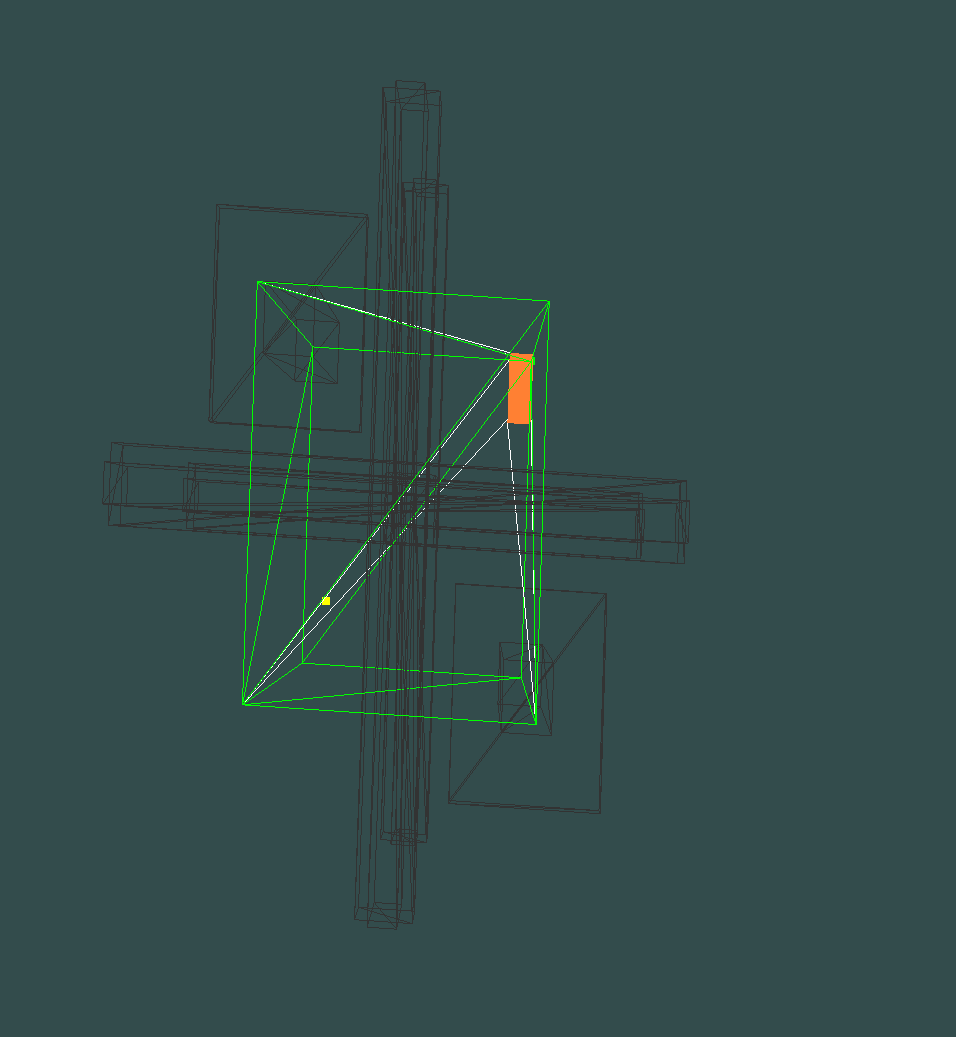
\includegraphics[width=0.3\linewidth]{clutter_top.png}
		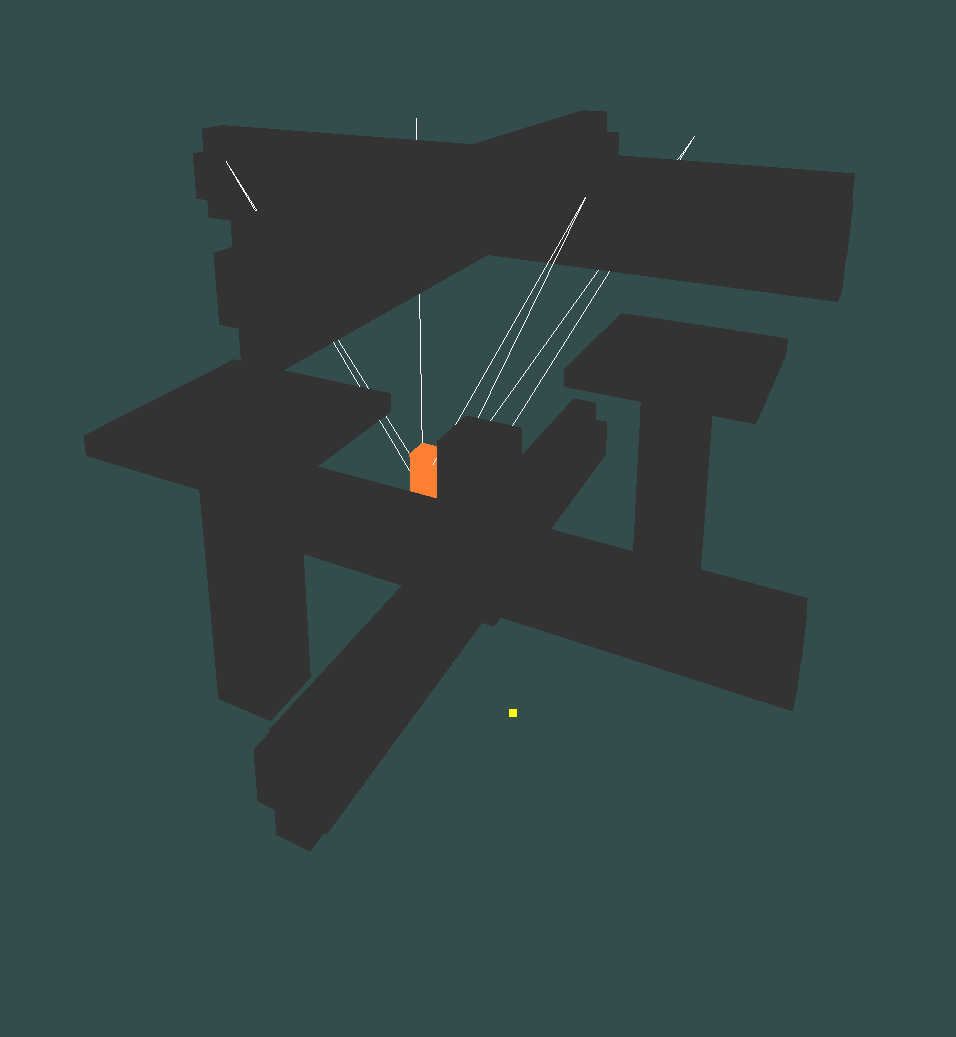
\includegraphics[width=0.3\linewidth]{clutter_perspective.png}
		\caption{Sample Planning Problem}
		\label{fig:sample_planning_problem}
	\end{figure}

	The software was asked to find a collision-free B-spline path of degree 8
	for the problem shown in Figure~\ref{fig:sample_planning_problem}. Different
	stages in the path-processing stage of the planning is reported in
	Figures~\ref{fig:sample_trajectory_after_simplification}
	and~\ref{fig:sample_trajectory_with_augmented_set_of_poses}.

	%\begin{figure}[hb]
	%	\centering
	%	\begin{minipage}{\linewidth}
	%		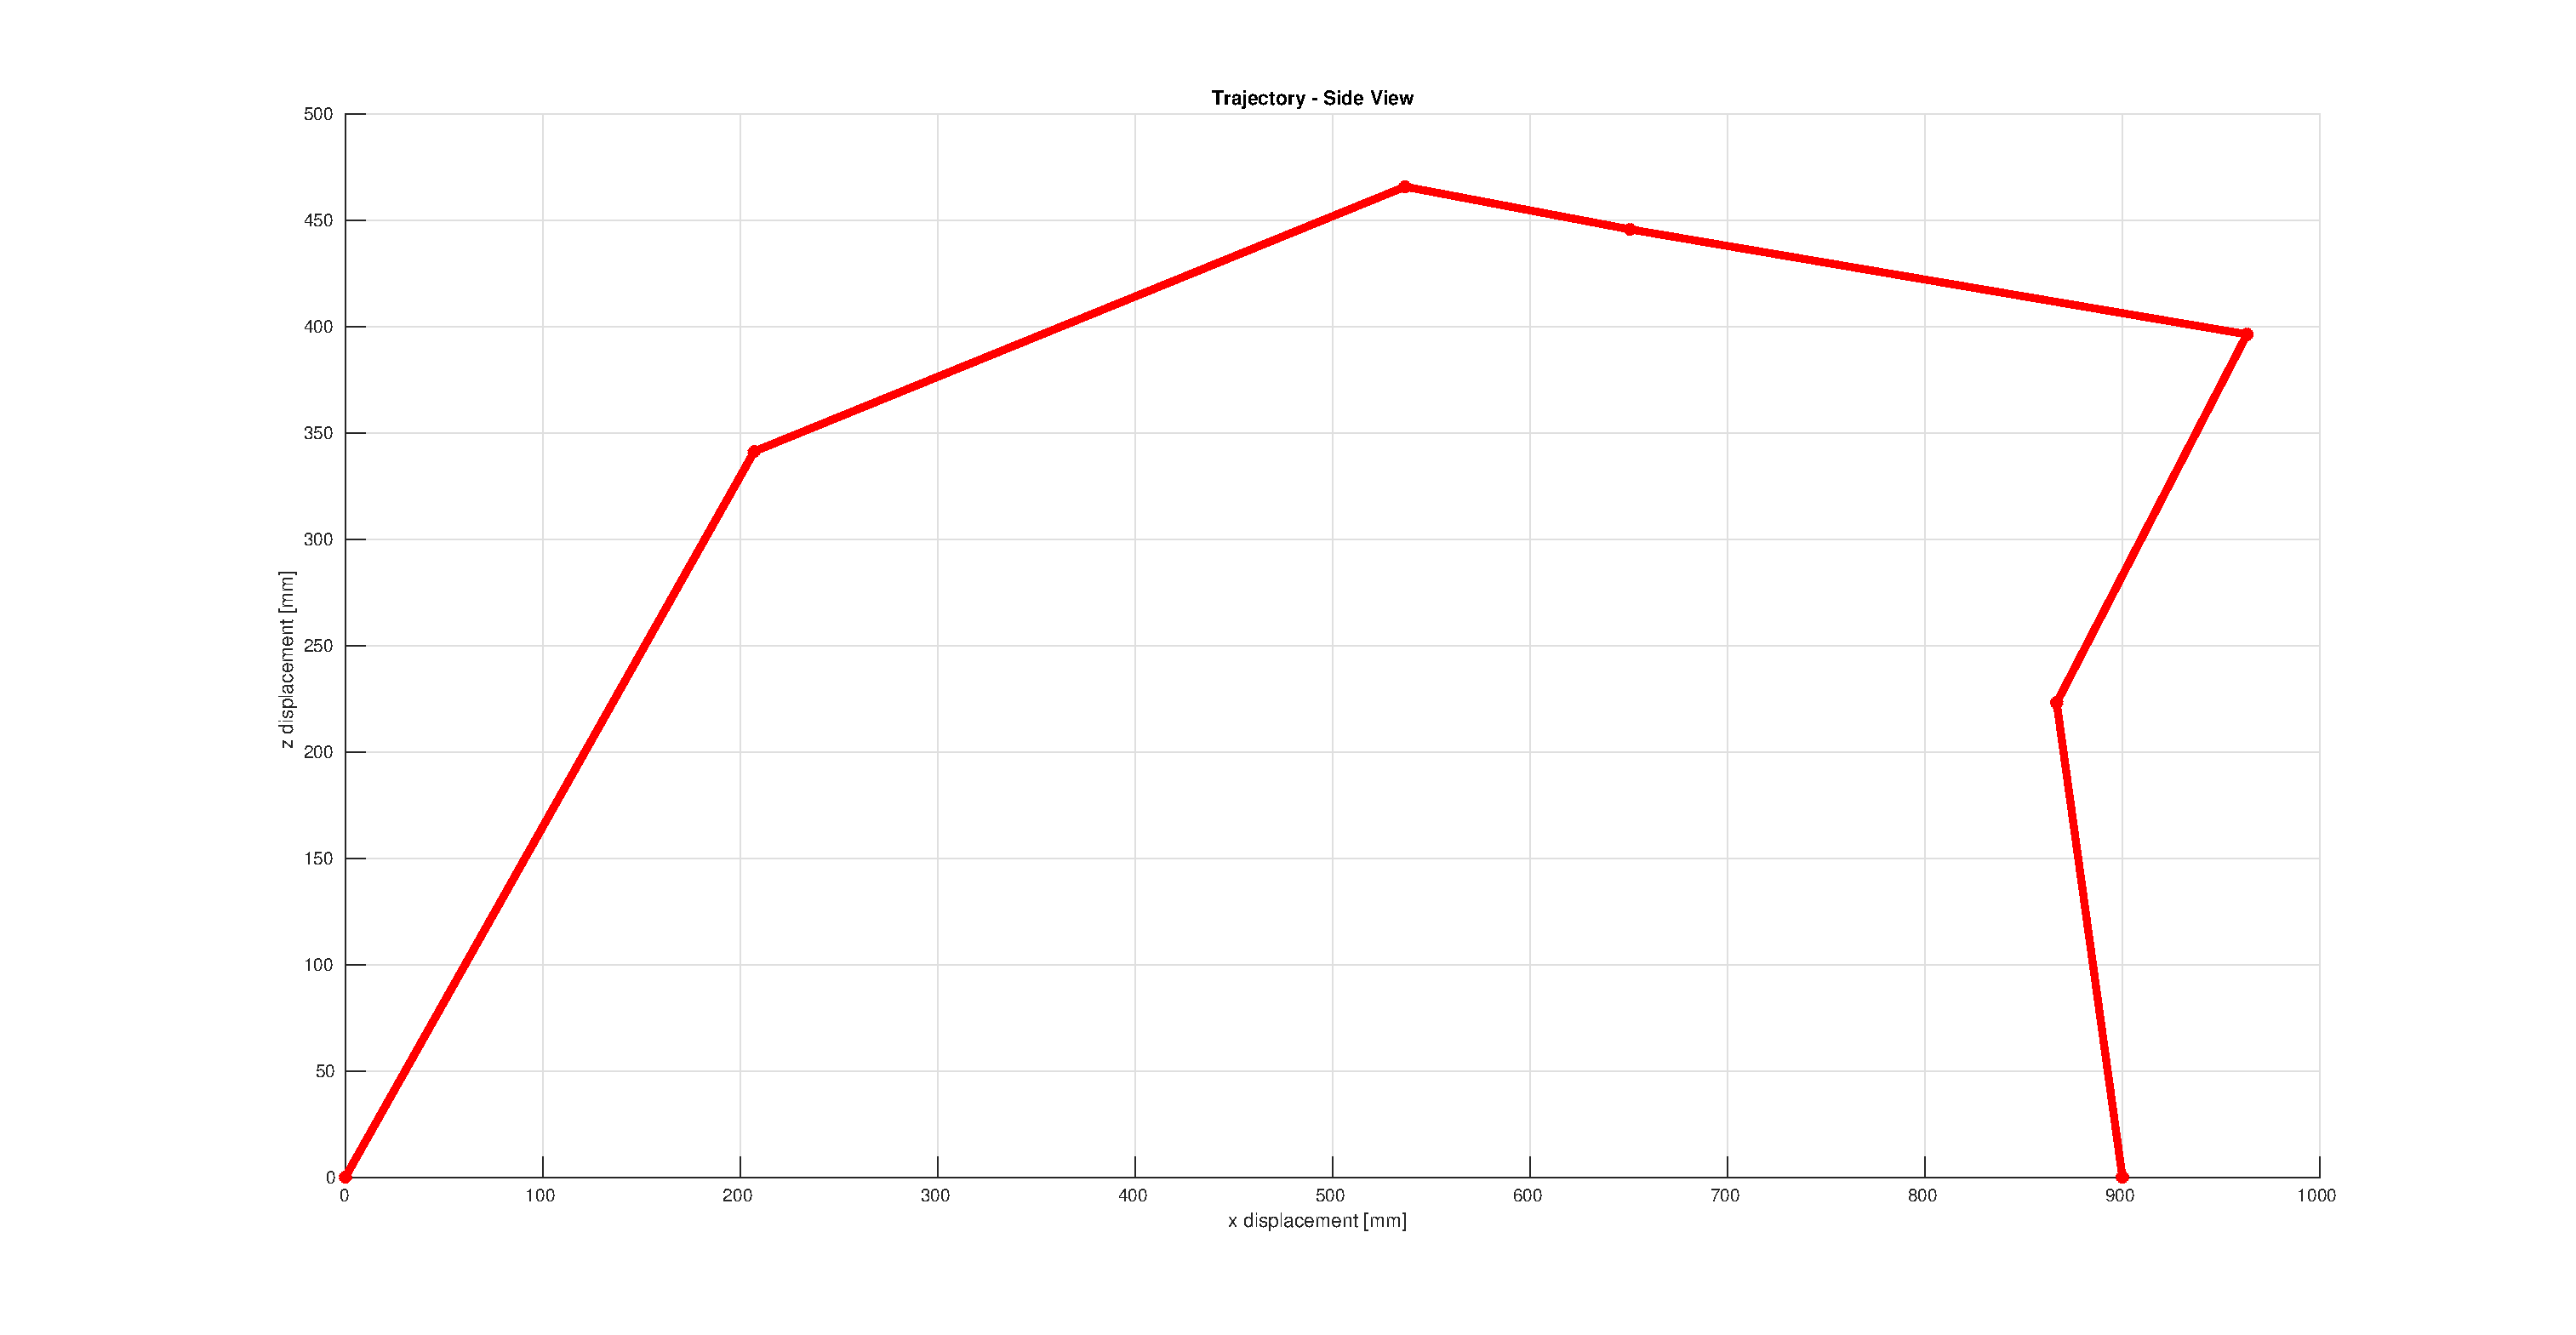
\includegraphics[height=0.45\linewidth, width=0.45\linewidth]{trajectory_no_simplify_side.eps}
	%		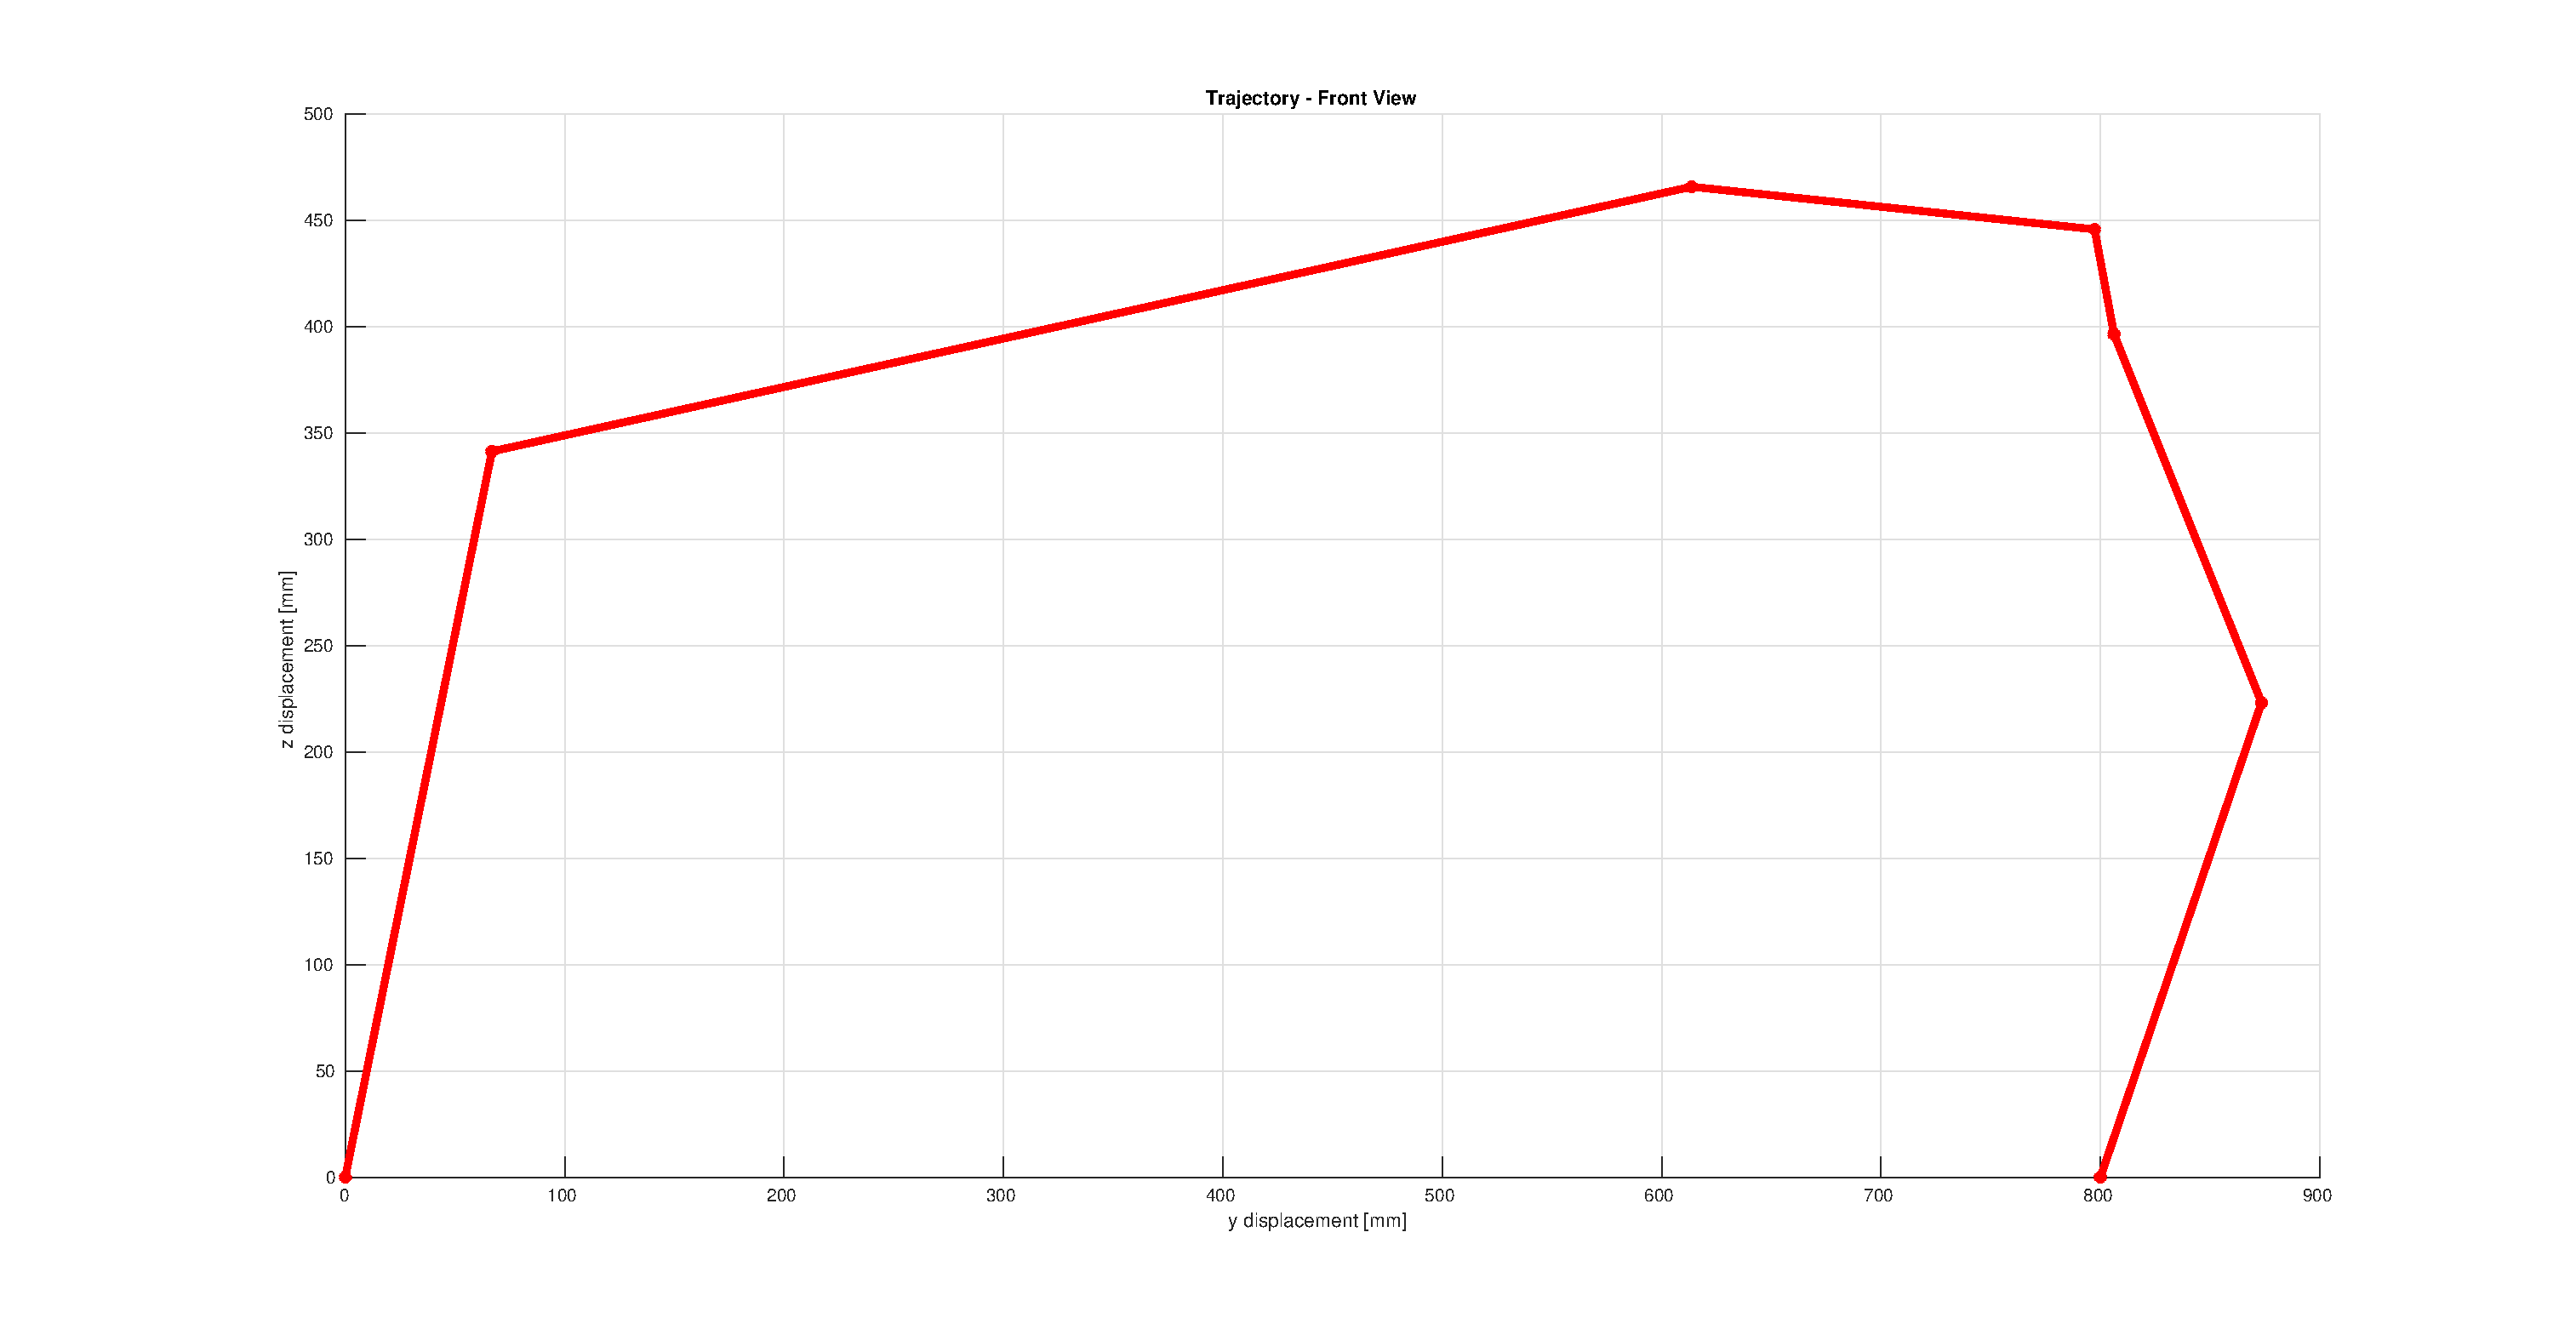
\includegraphics[height=0.45\linewidth, width=0.45\linewidth]{trajectory_no_simplify_front.eps}
	%		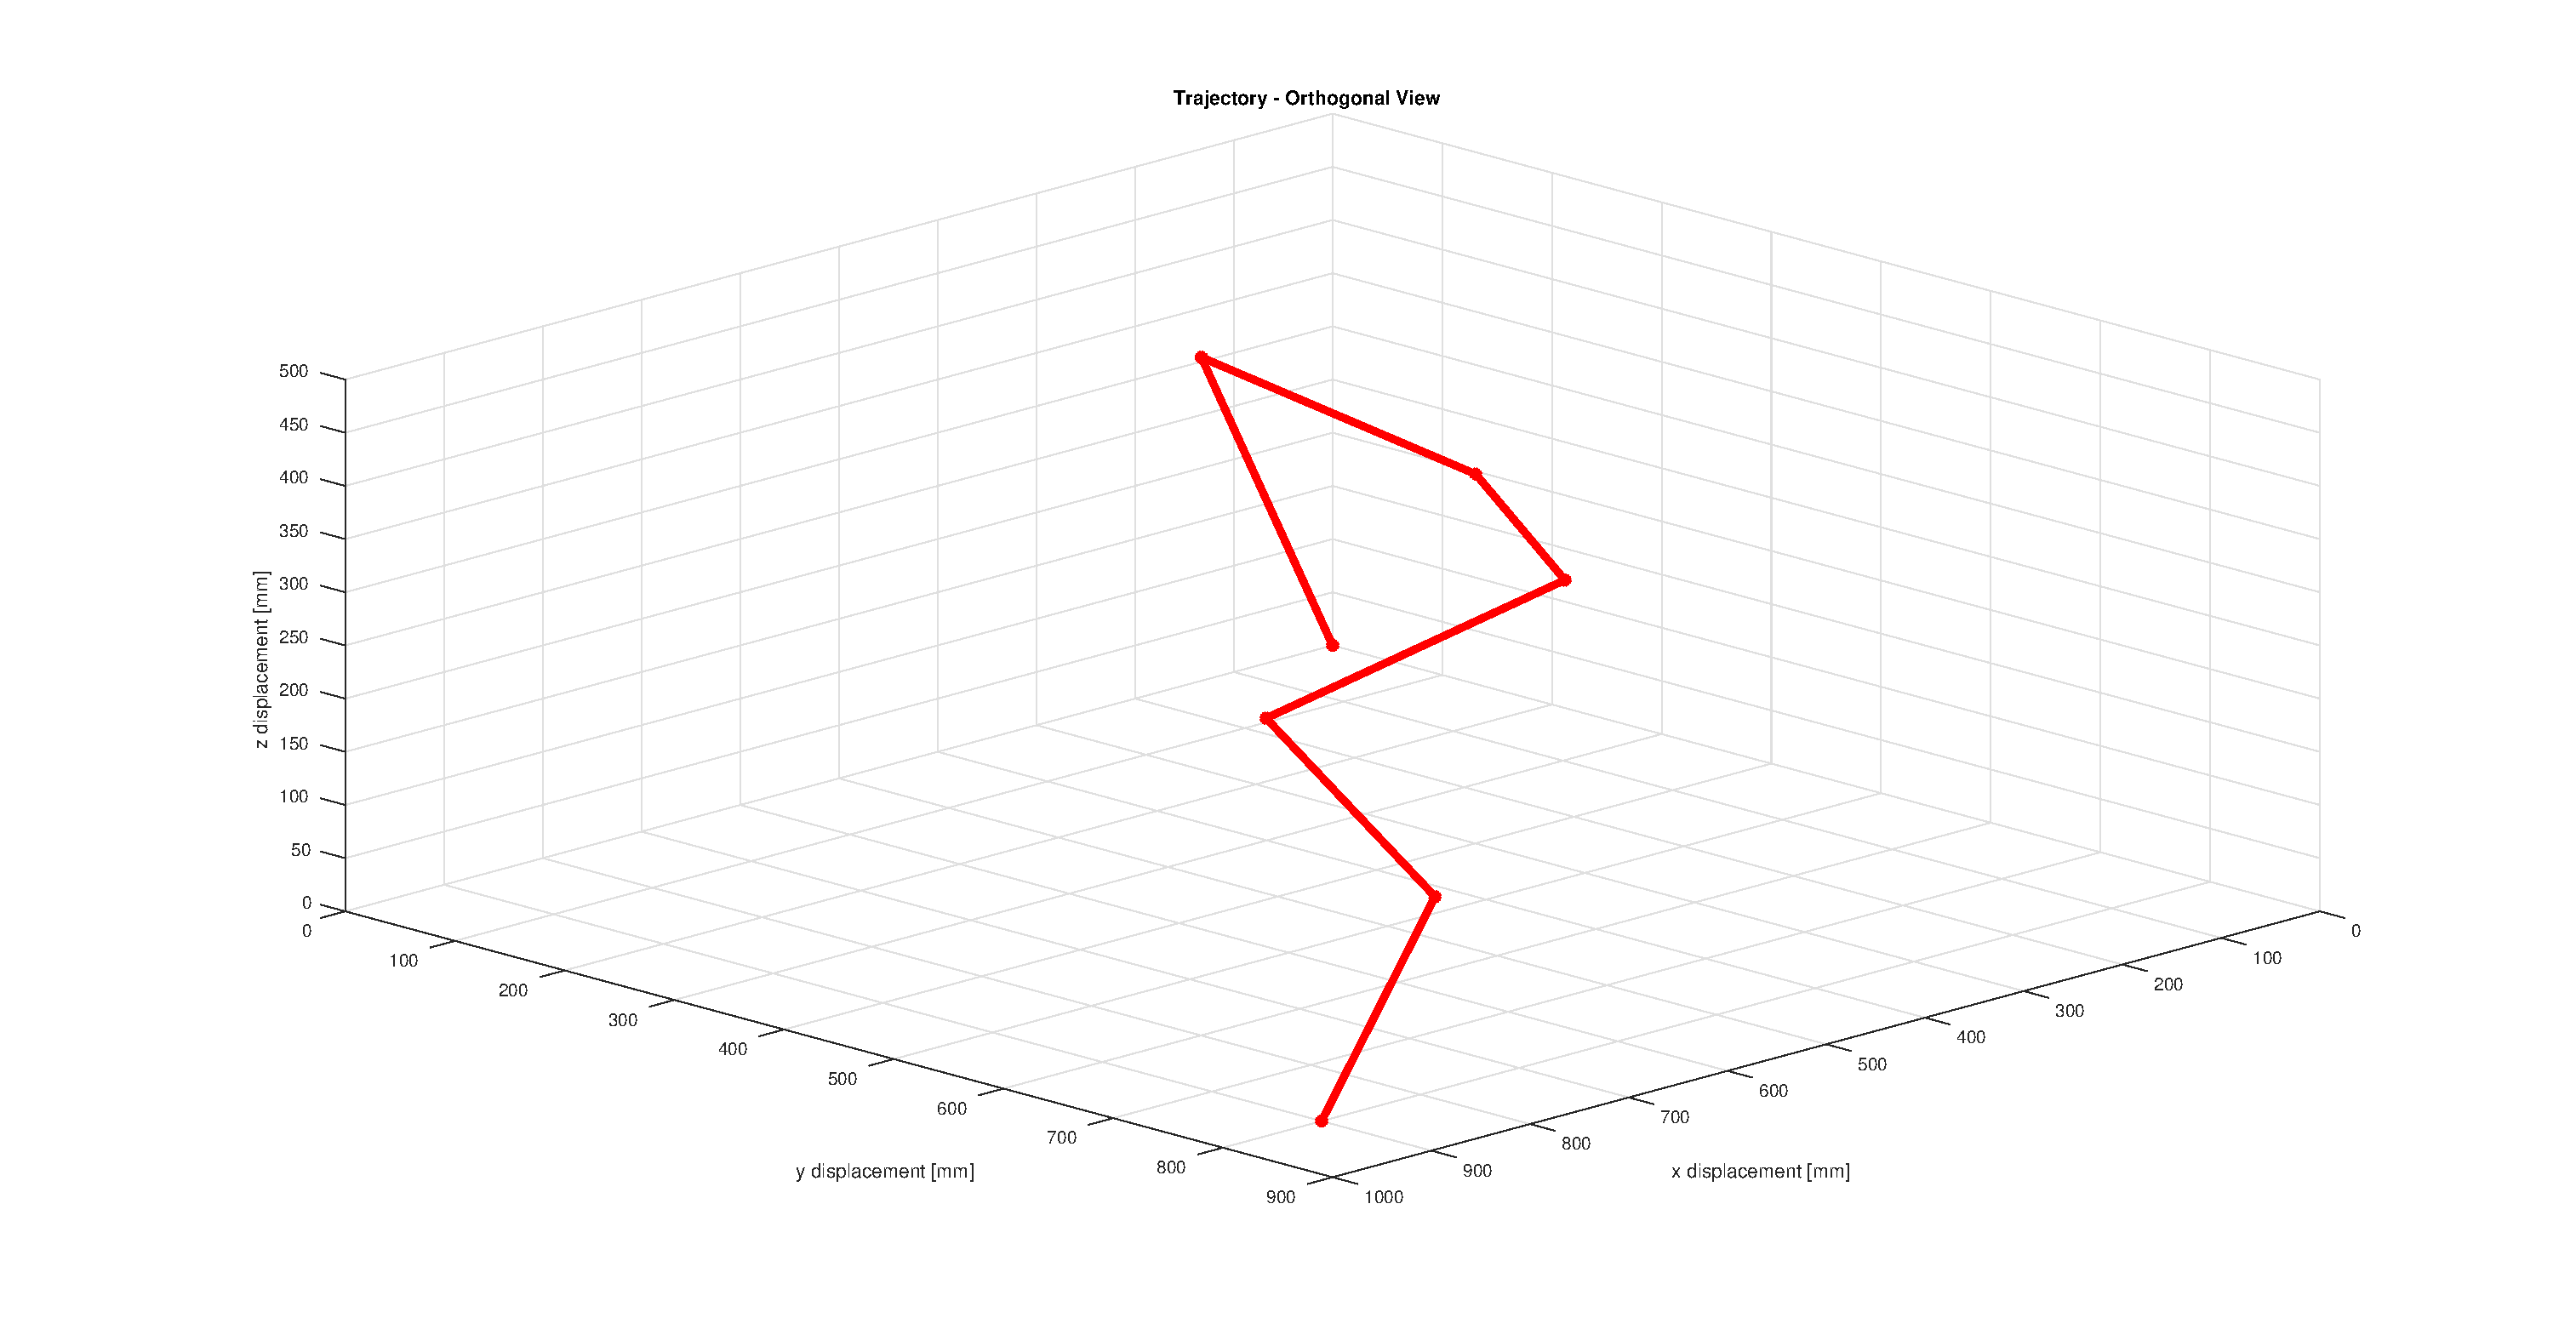
\includegraphics[height=0.45\linewidth, width=0.45\linewidth]{trajectory_no_simplify_orthogonal.eps}
	%		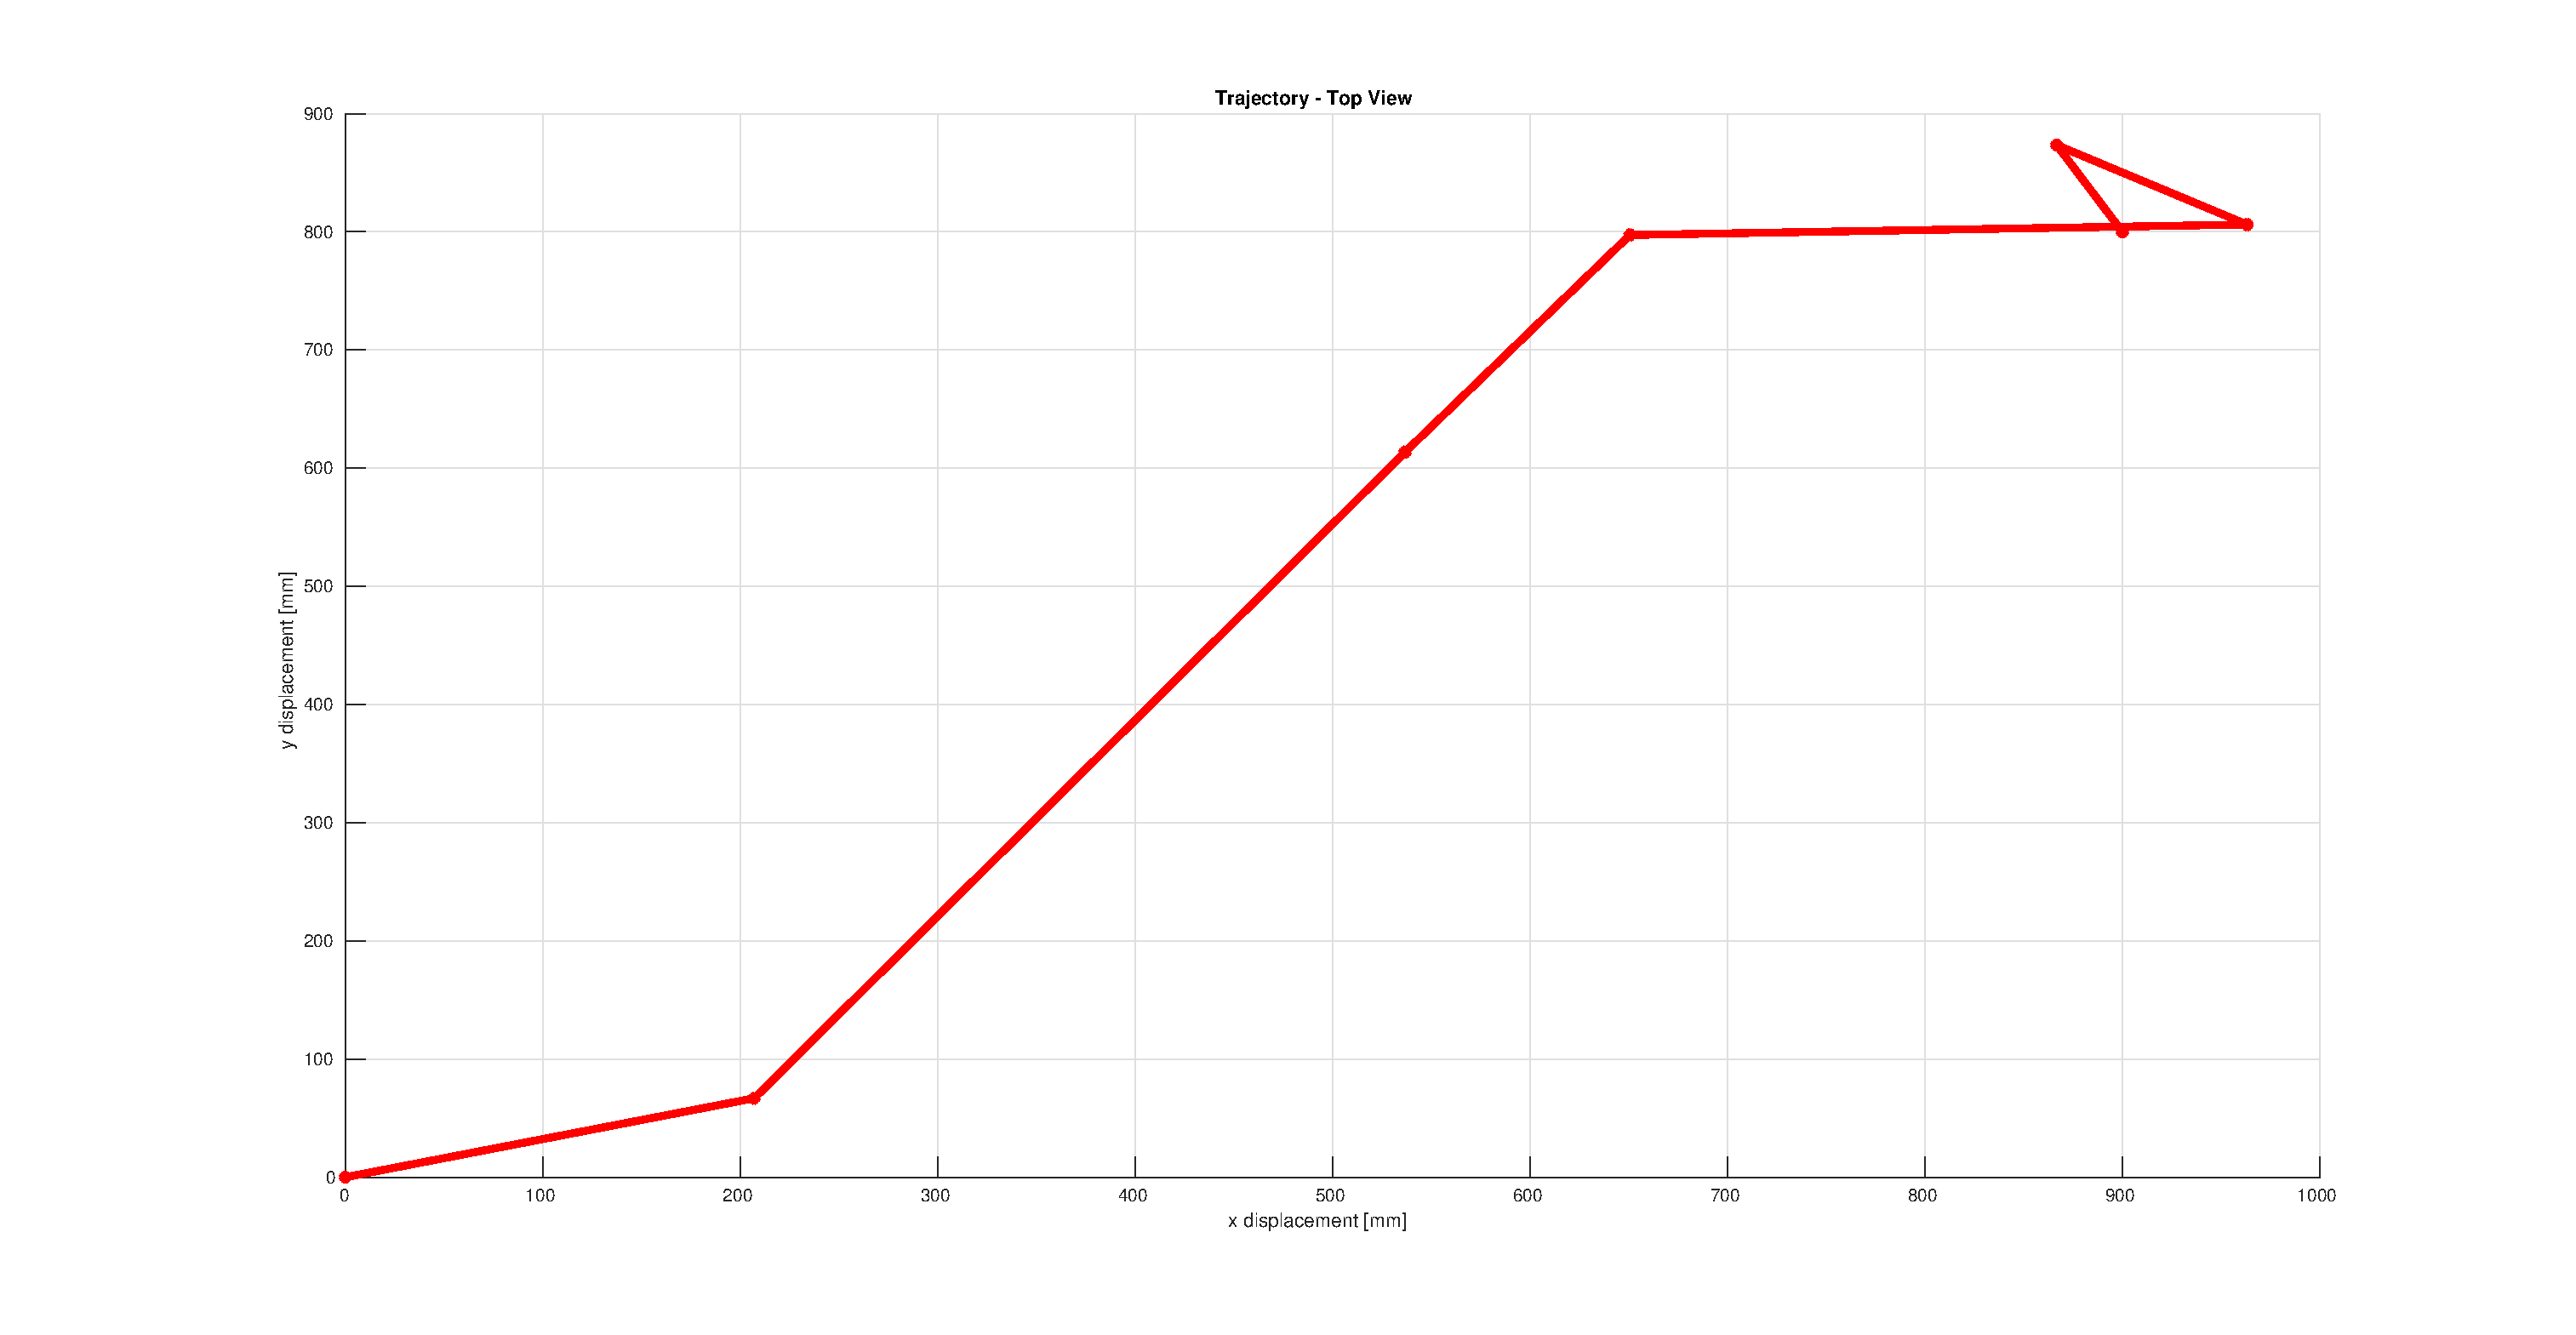
\includegraphics[height=0.45\linewidth, width=0.45\linewidth]{trajectory_no_simplify_top.eps}
	%	\end{minipage}
	%	\caption{Sample Trajectory Before Simplification}
	%\end{figure}

	\begin{figure}[hb]
		\centering
		\begin{minipage}{0.8\linewidth}
			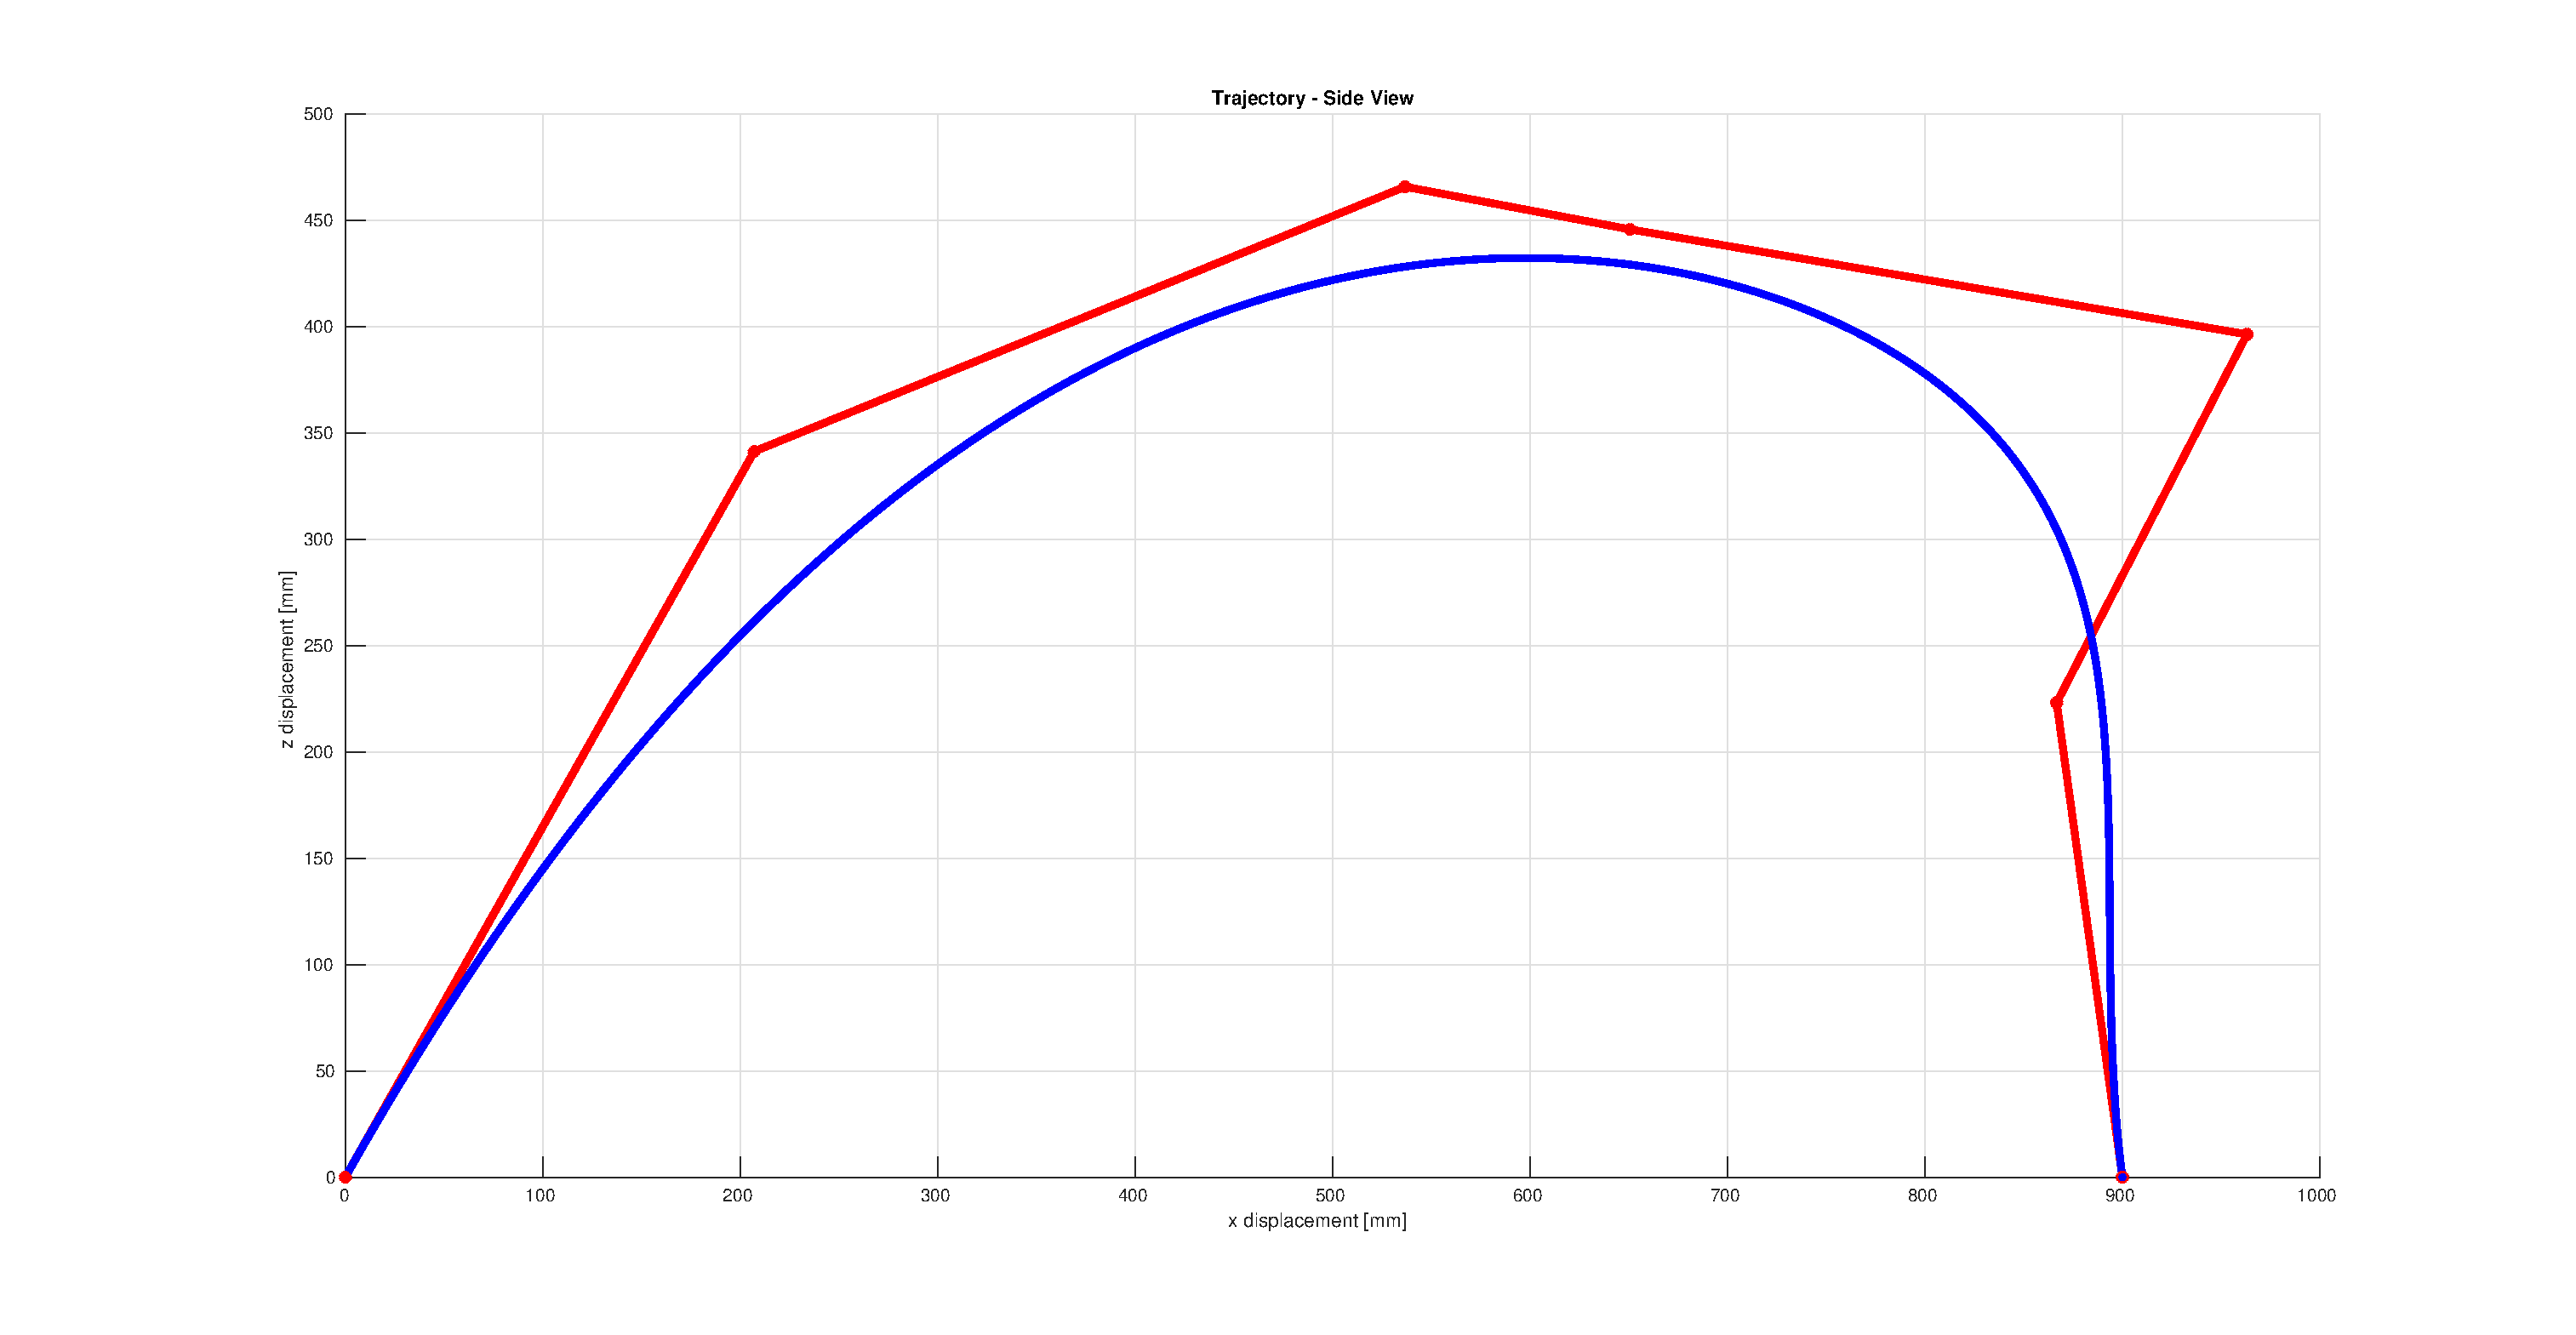
\includegraphics[height=0.45\linewidth, width=0.45\linewidth]{trajectory_simplify_no_subdivide_side.eps}
			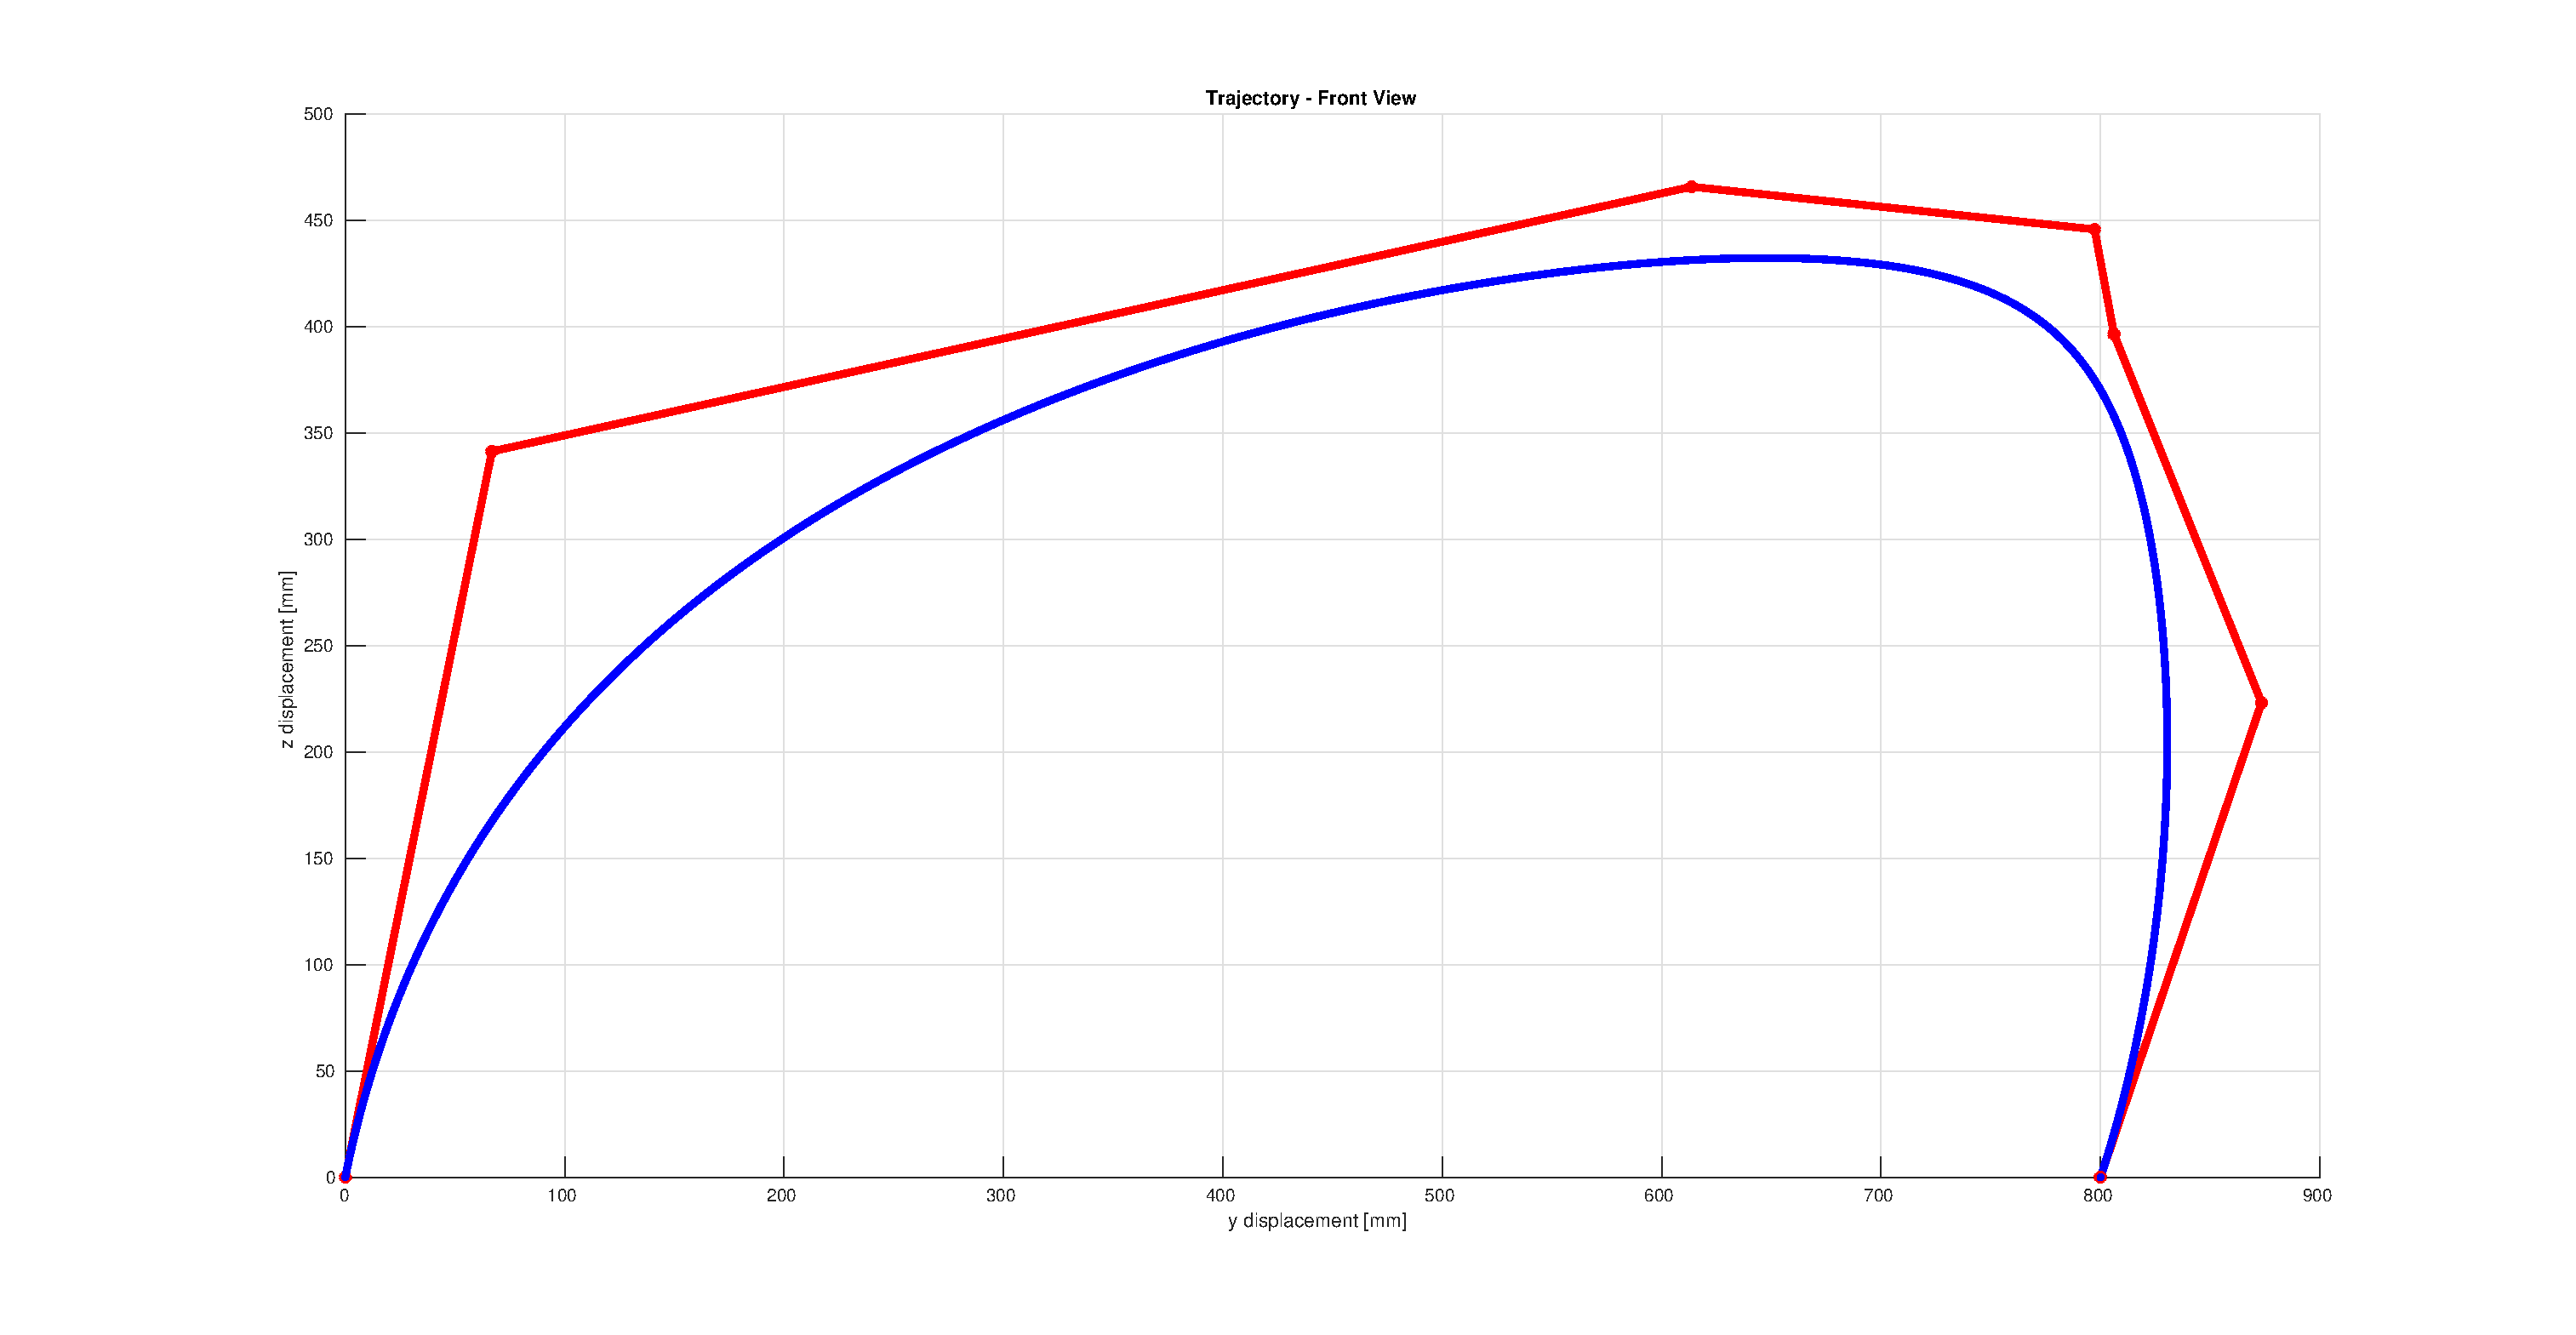
\includegraphics[height=0.45\linewidth, width=0.45\linewidth]{trajectory_simplify_no_subdivide_front.eps}
			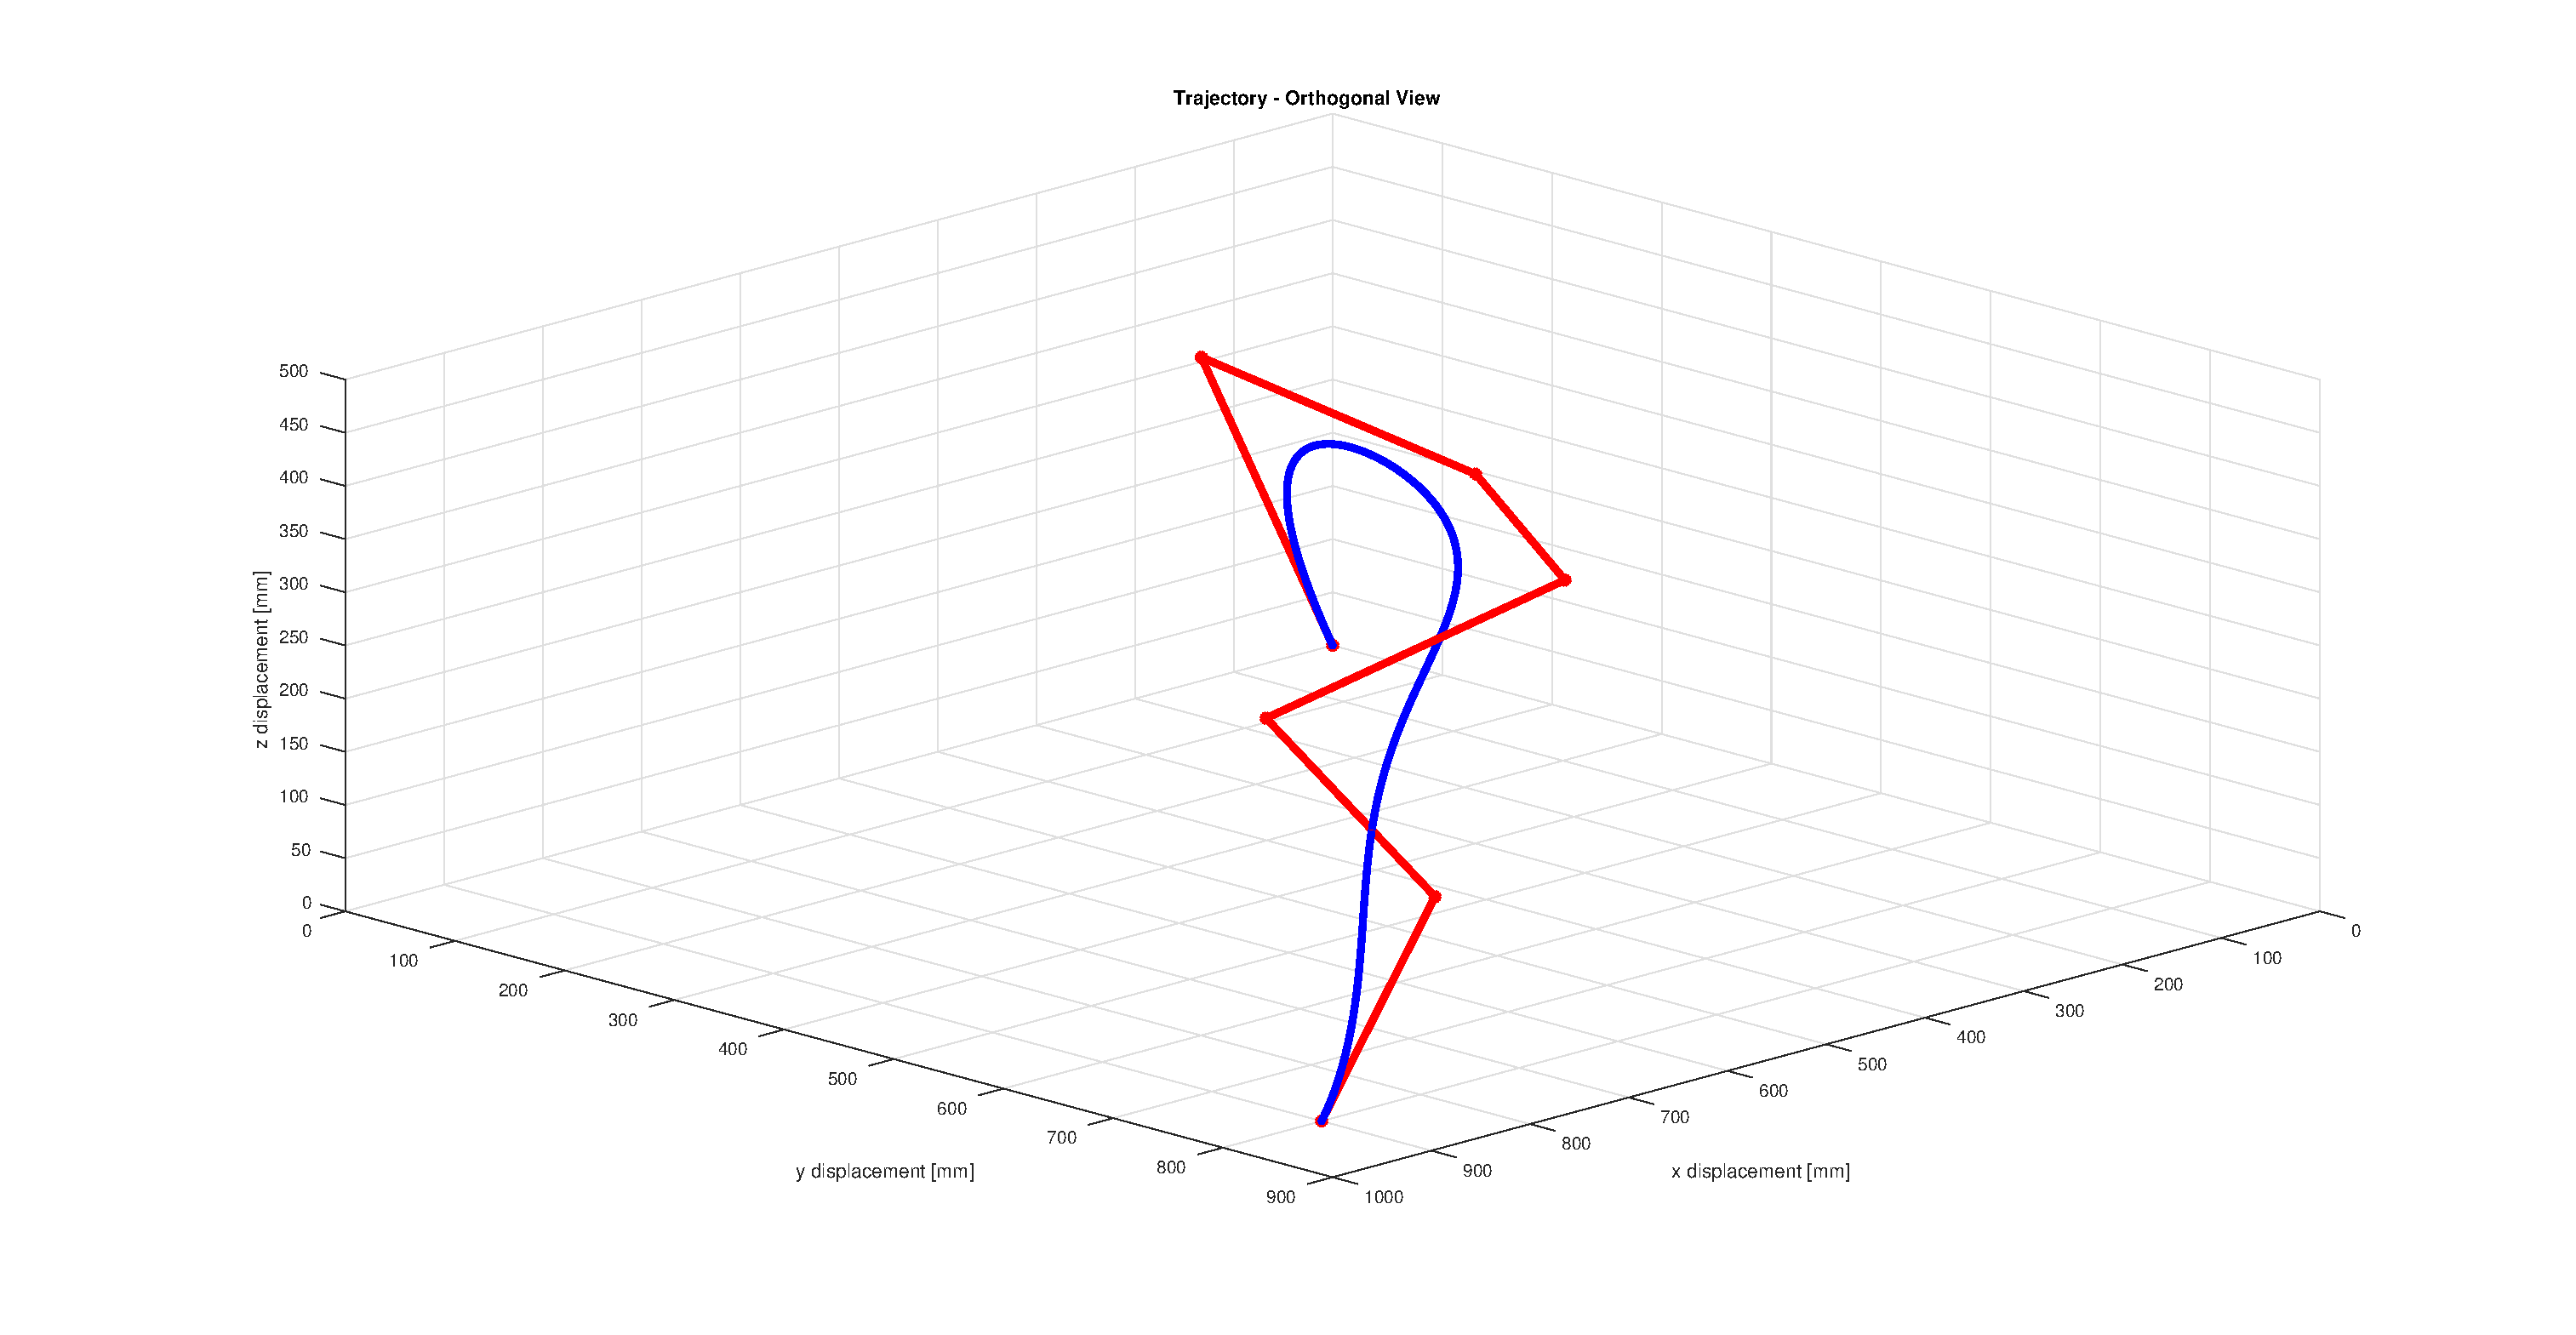
\includegraphics[height=0.45\linewidth, width=0.45\linewidth]{trajectory_simplify_no_subdivide_orthogonal.eps}
			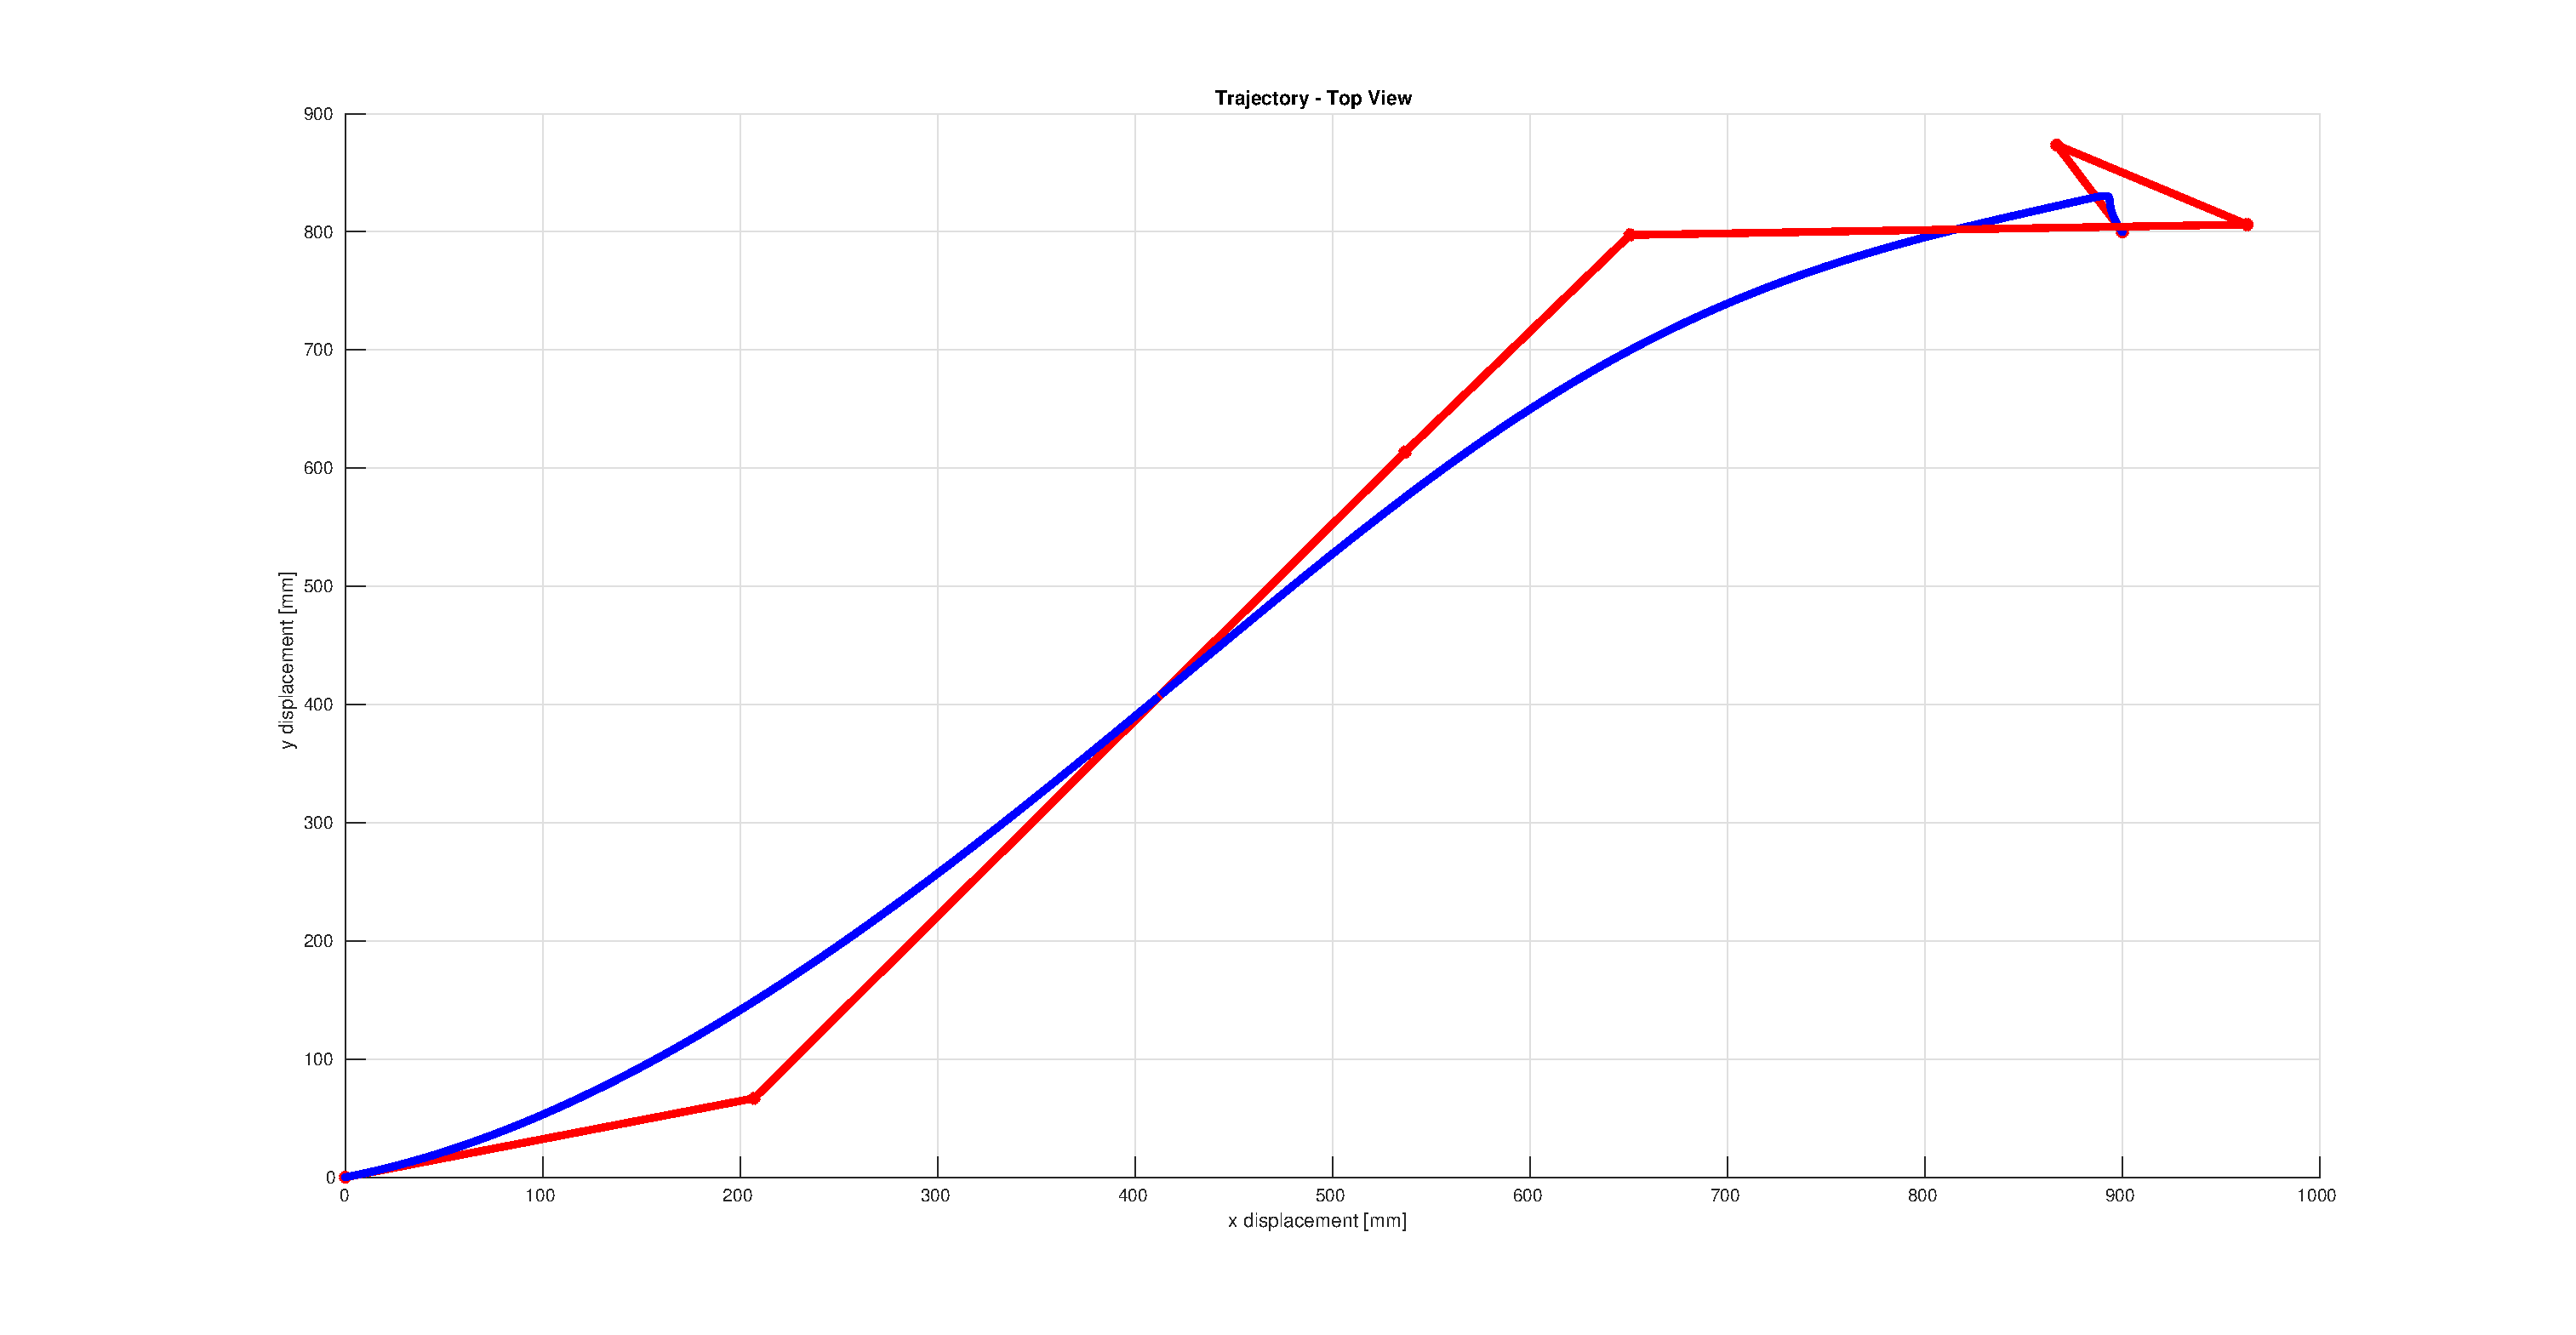
\includegraphics[height=0.45\linewidth, width=0.45\linewidth]{trajectory_simplify_no_subdivide_top.eps}
		\end{minipage}
		\caption{Sample Trajectory without Augmenting $\setofposes$}
		\label{fig:sample_trajectory_after_simplification}
	\end{figure}


	\begin{figure}[hb]
		\centering
		\begin{minipage}{0.8\linewidth}
			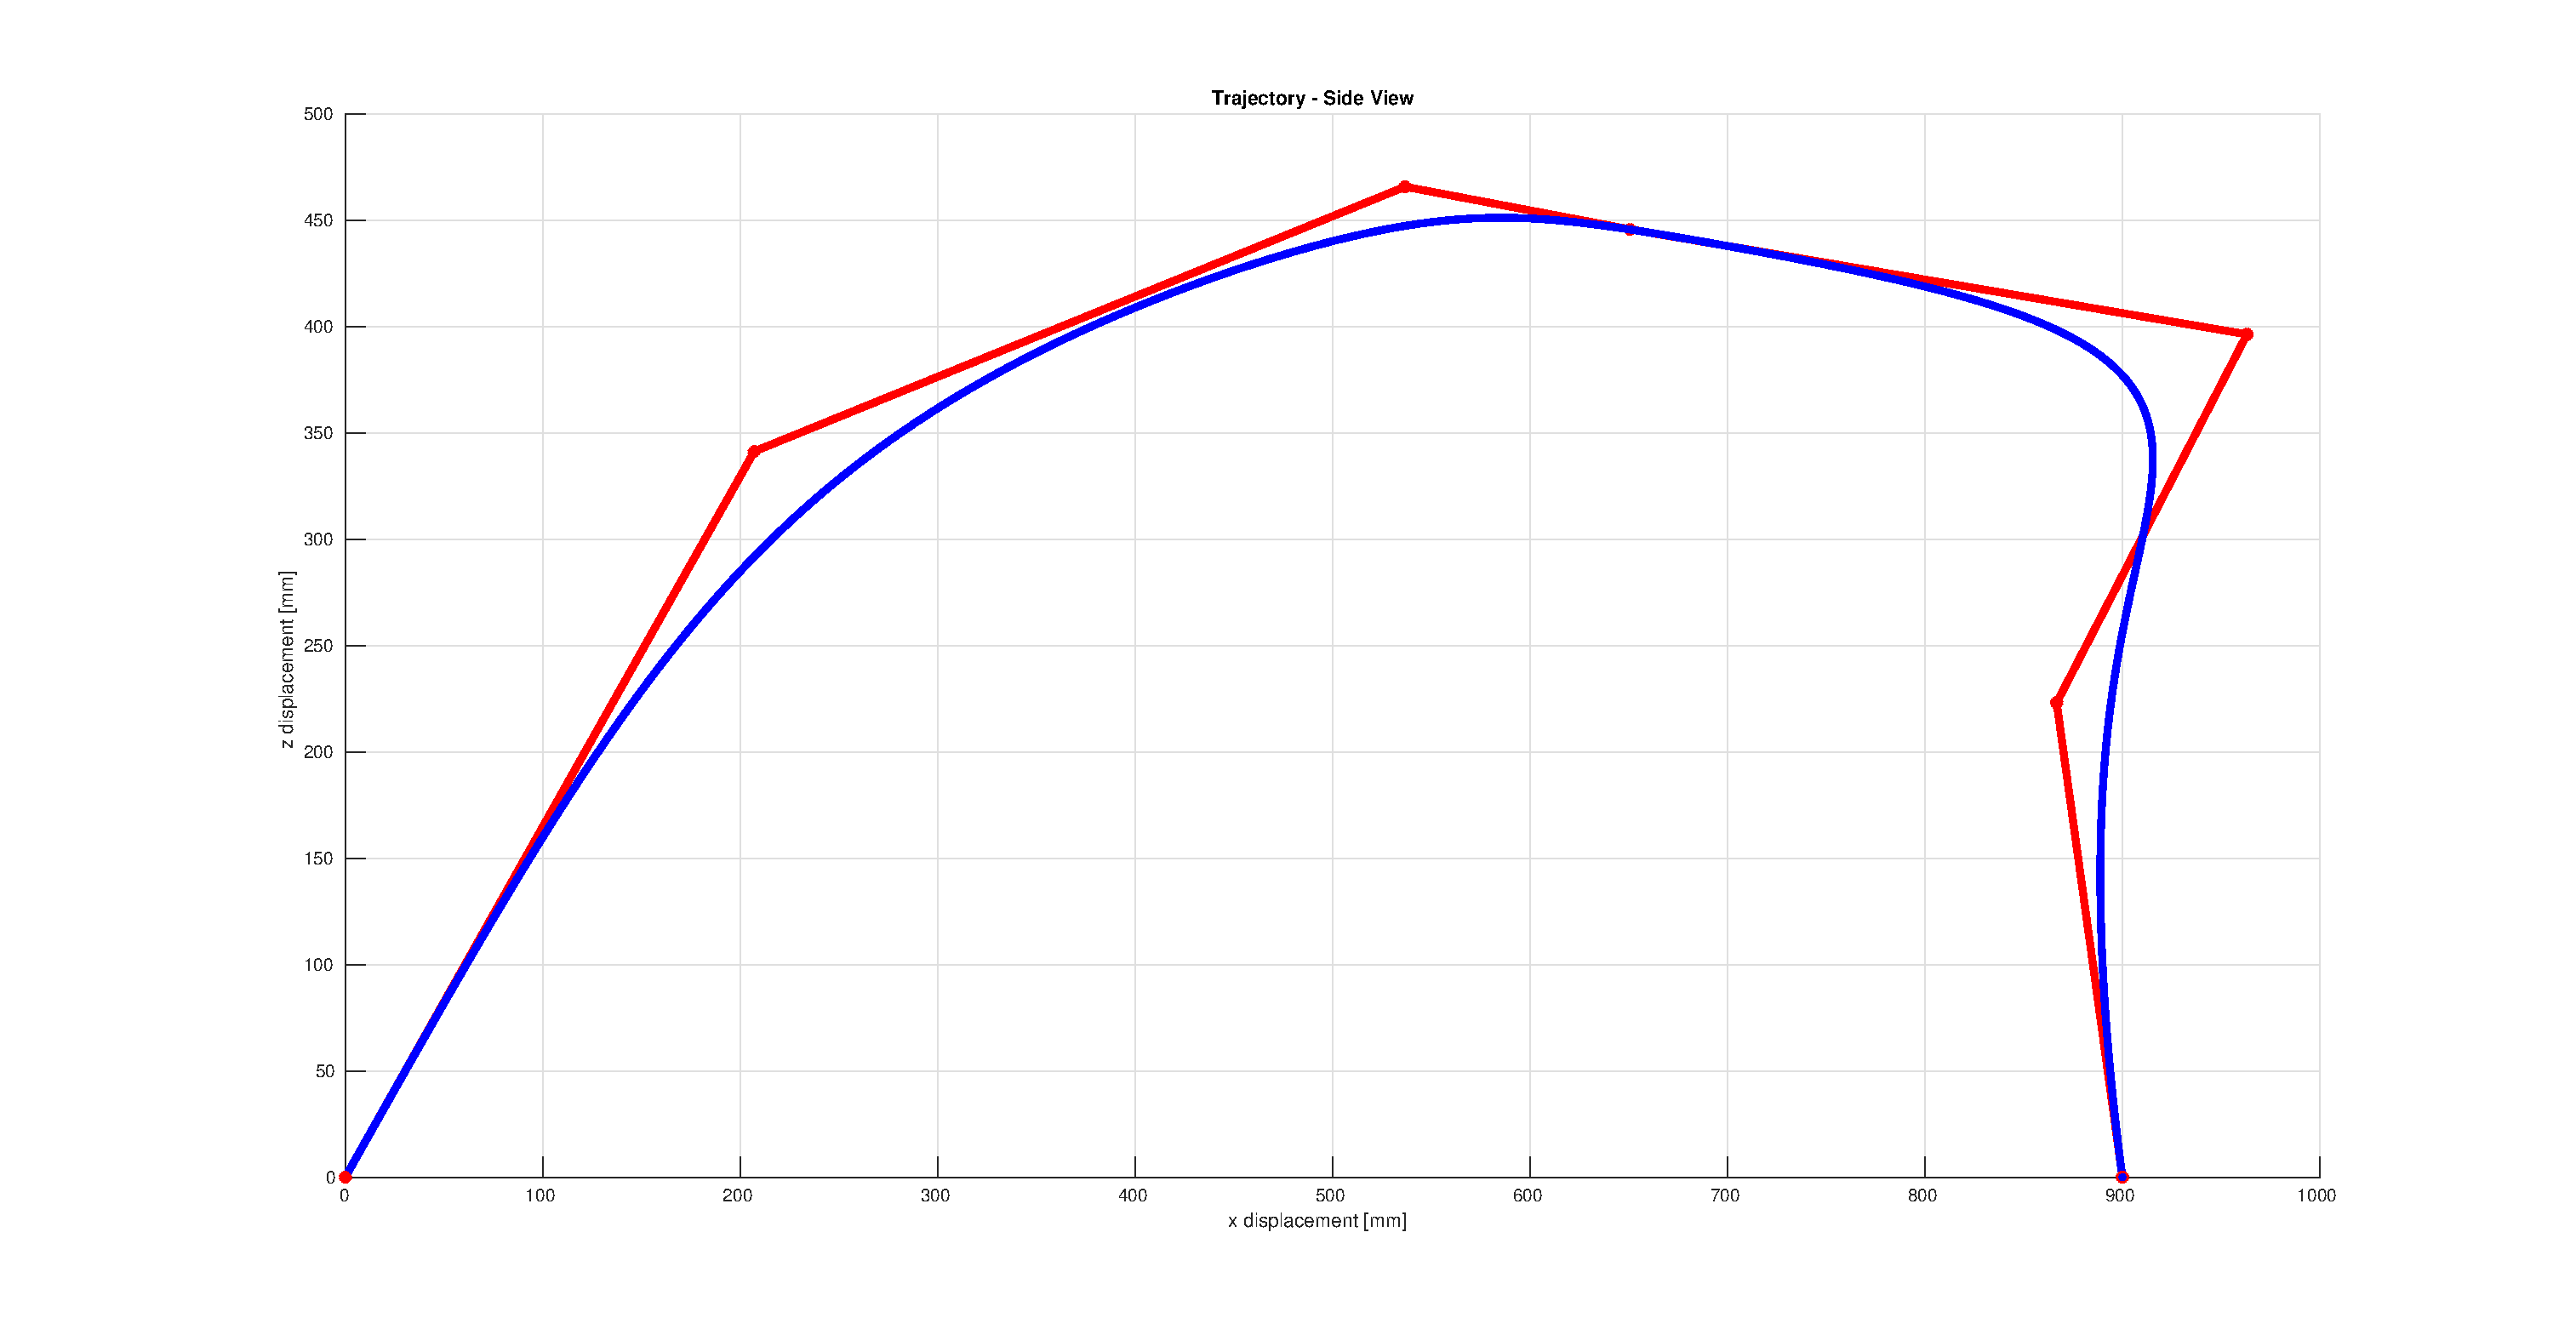
\includegraphics[height=0.45\linewidth, width=0.45\linewidth]{trajectory_simplify_subdivide_side.eps}
			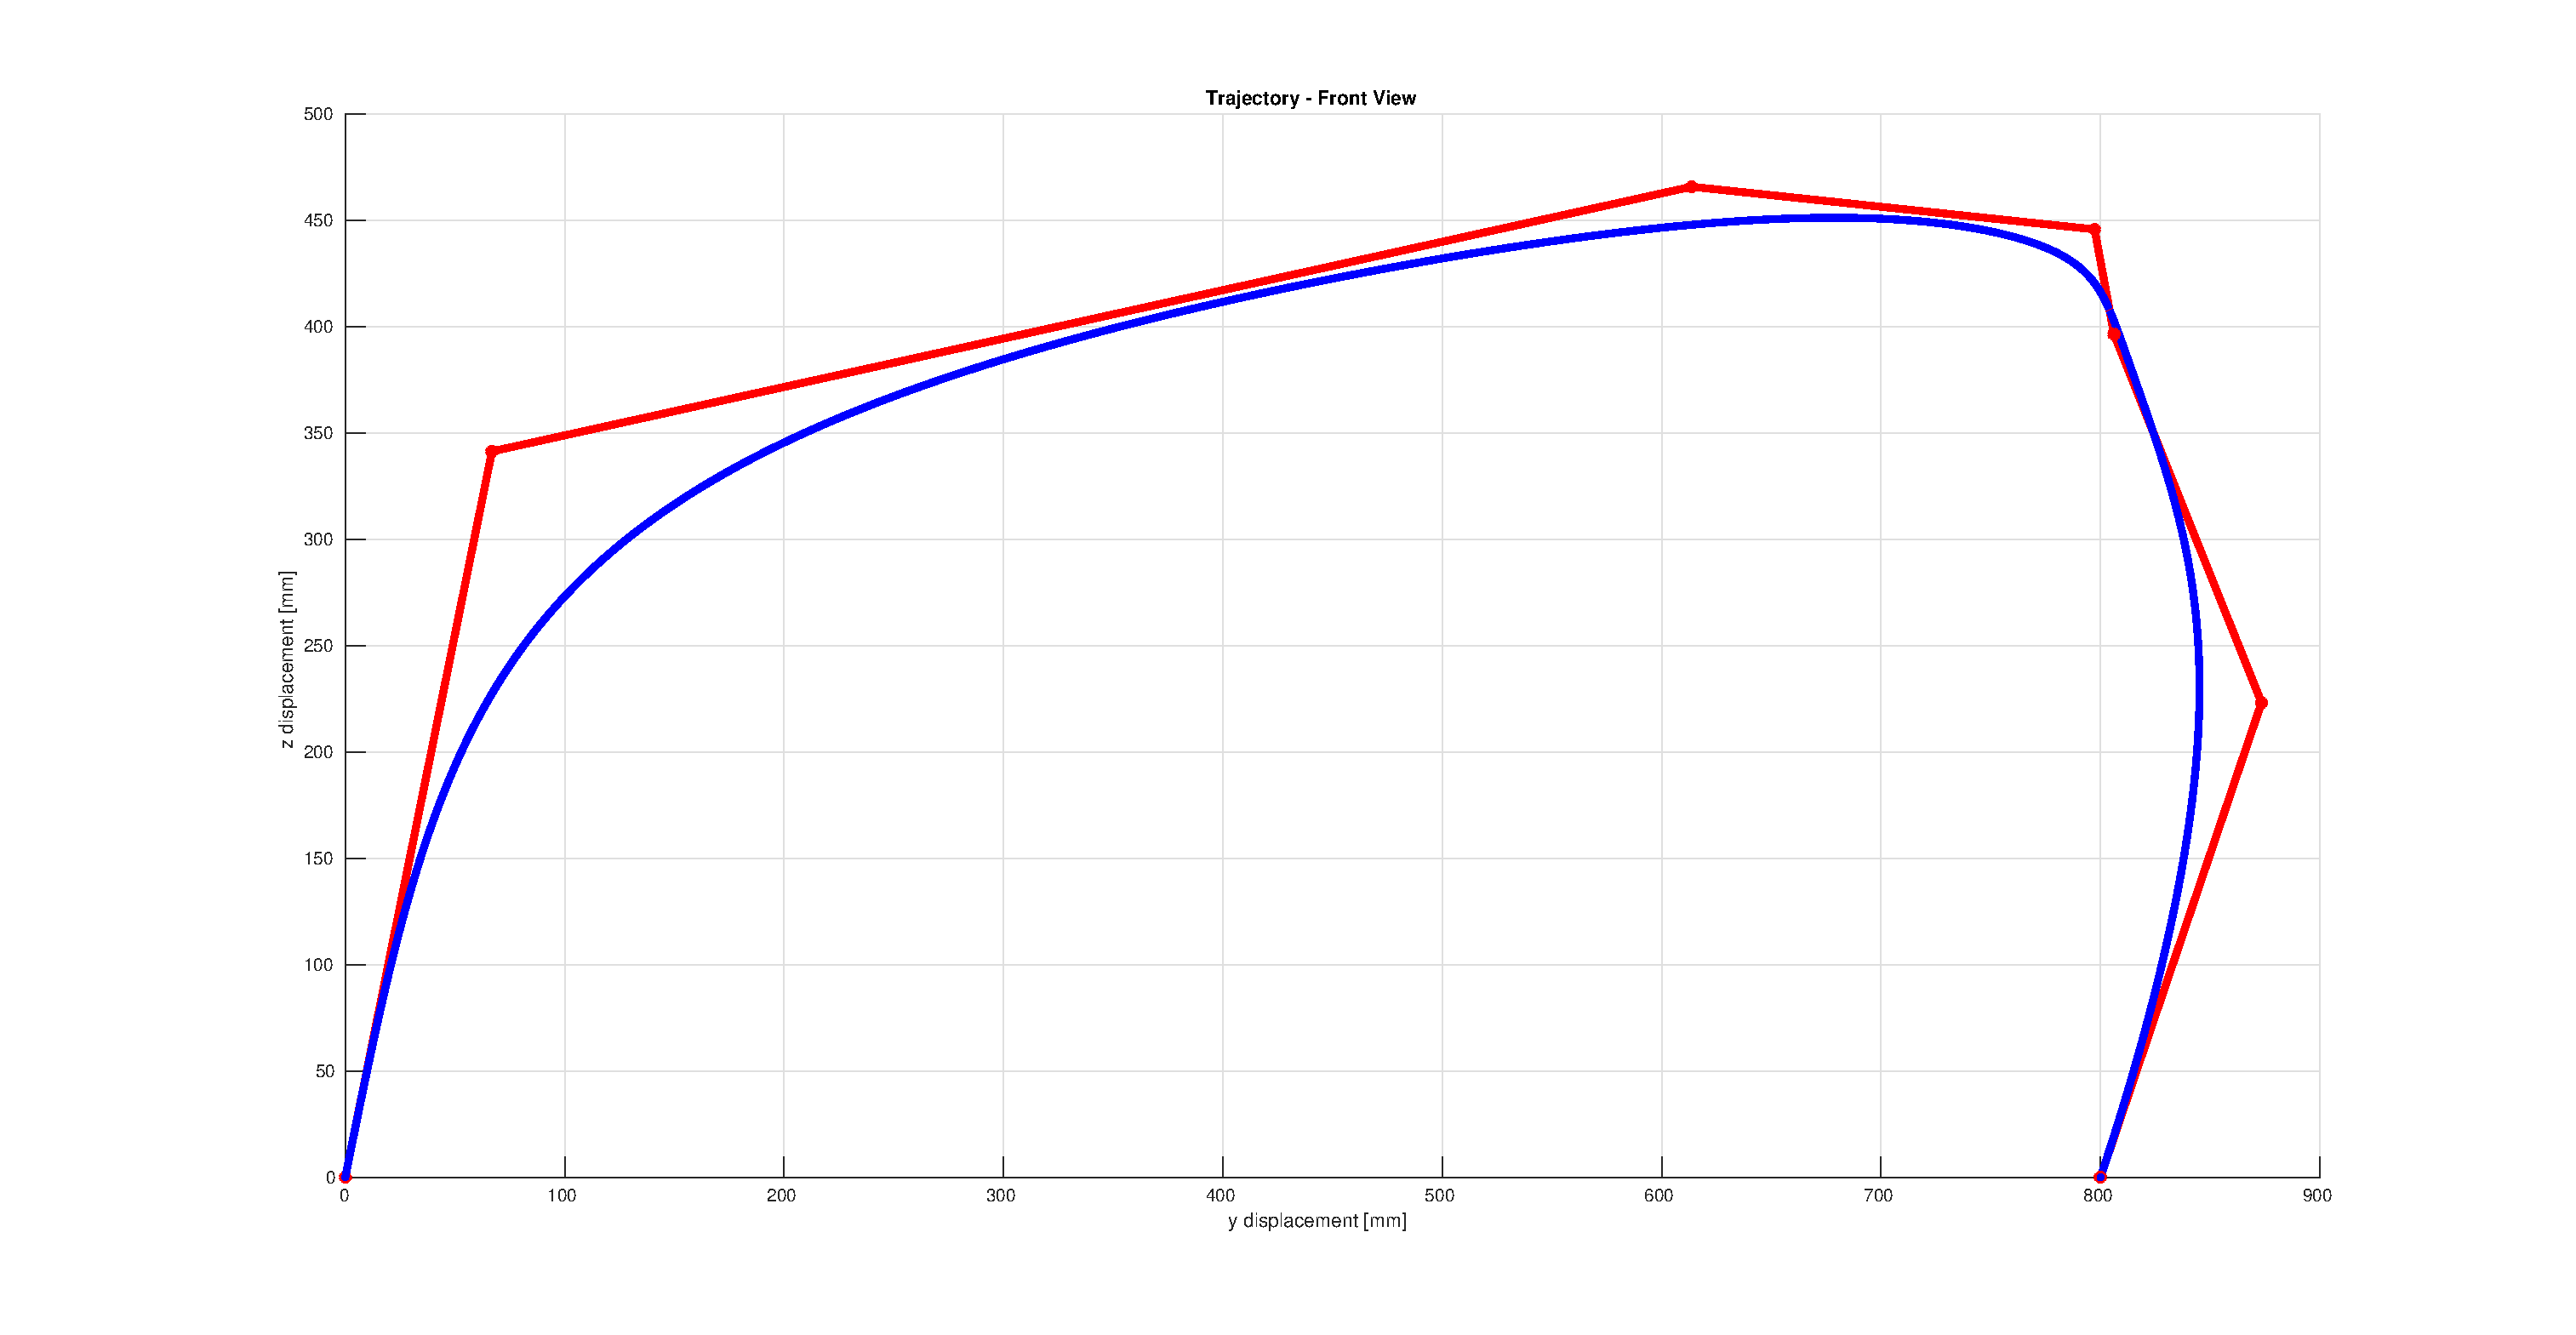
\includegraphics[height=0.45\linewidth, width=0.45\linewidth]{trajectory_simplify_subdivide_front.eps}
			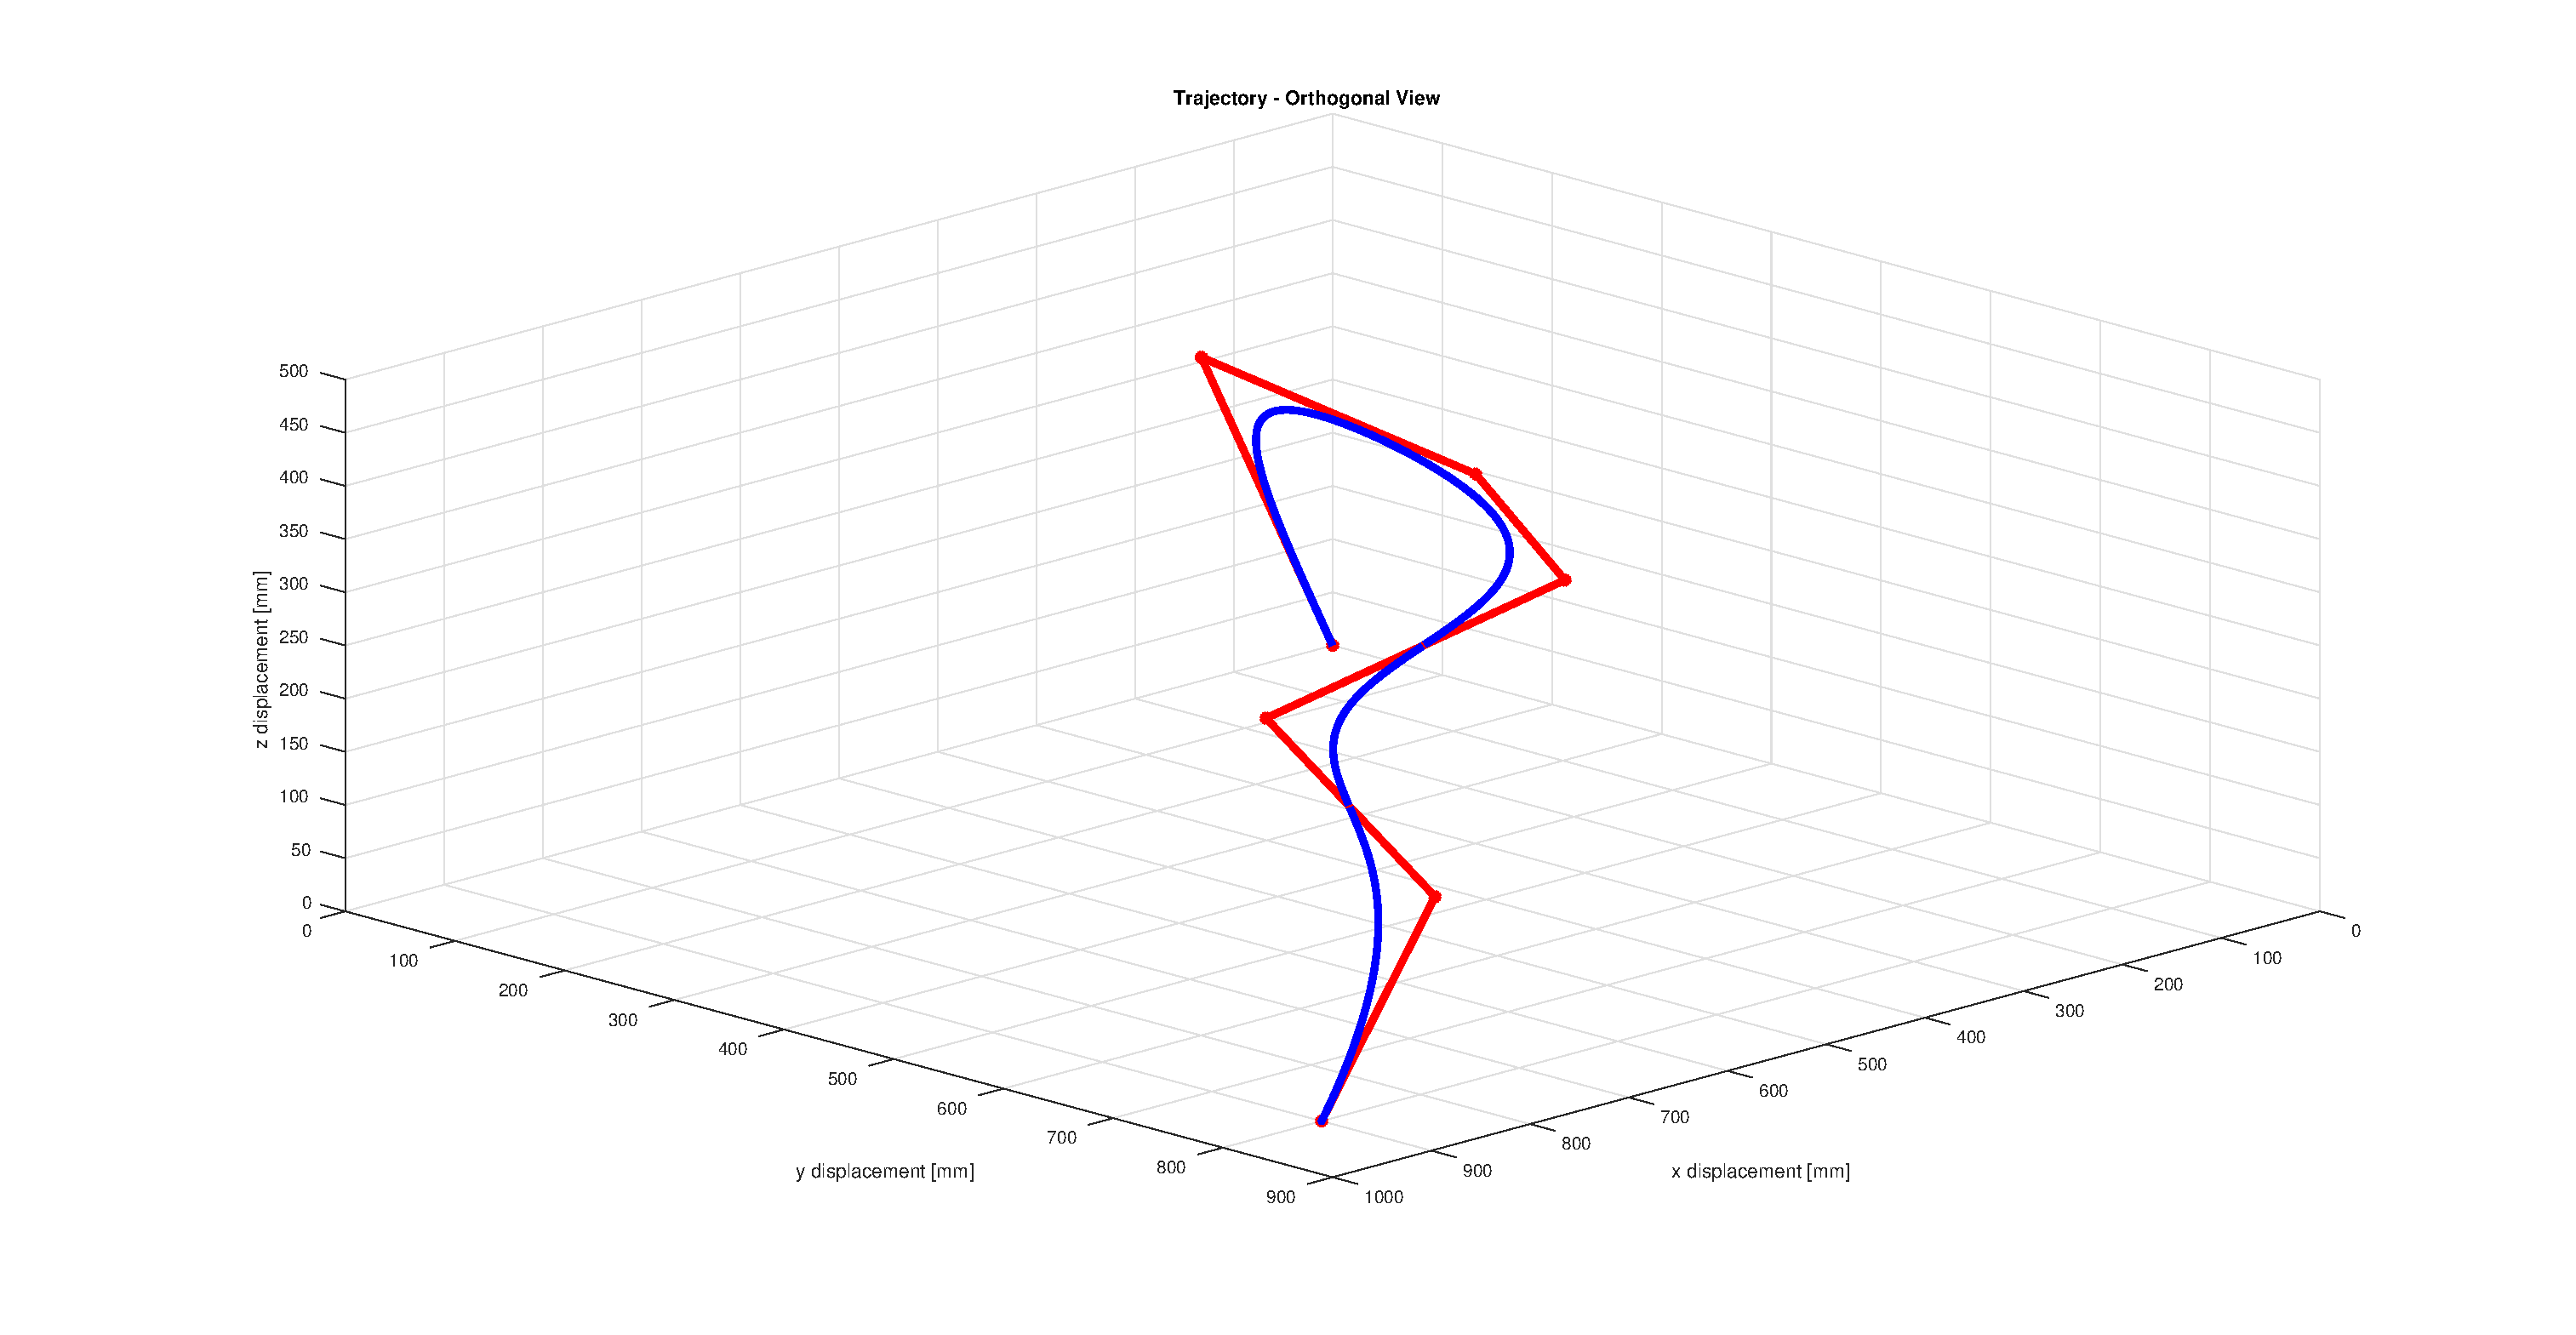
\includegraphics[height=0.45\linewidth, width=0.45\linewidth]{trajectory_simplify_subdivide_orthogonal.eps}
			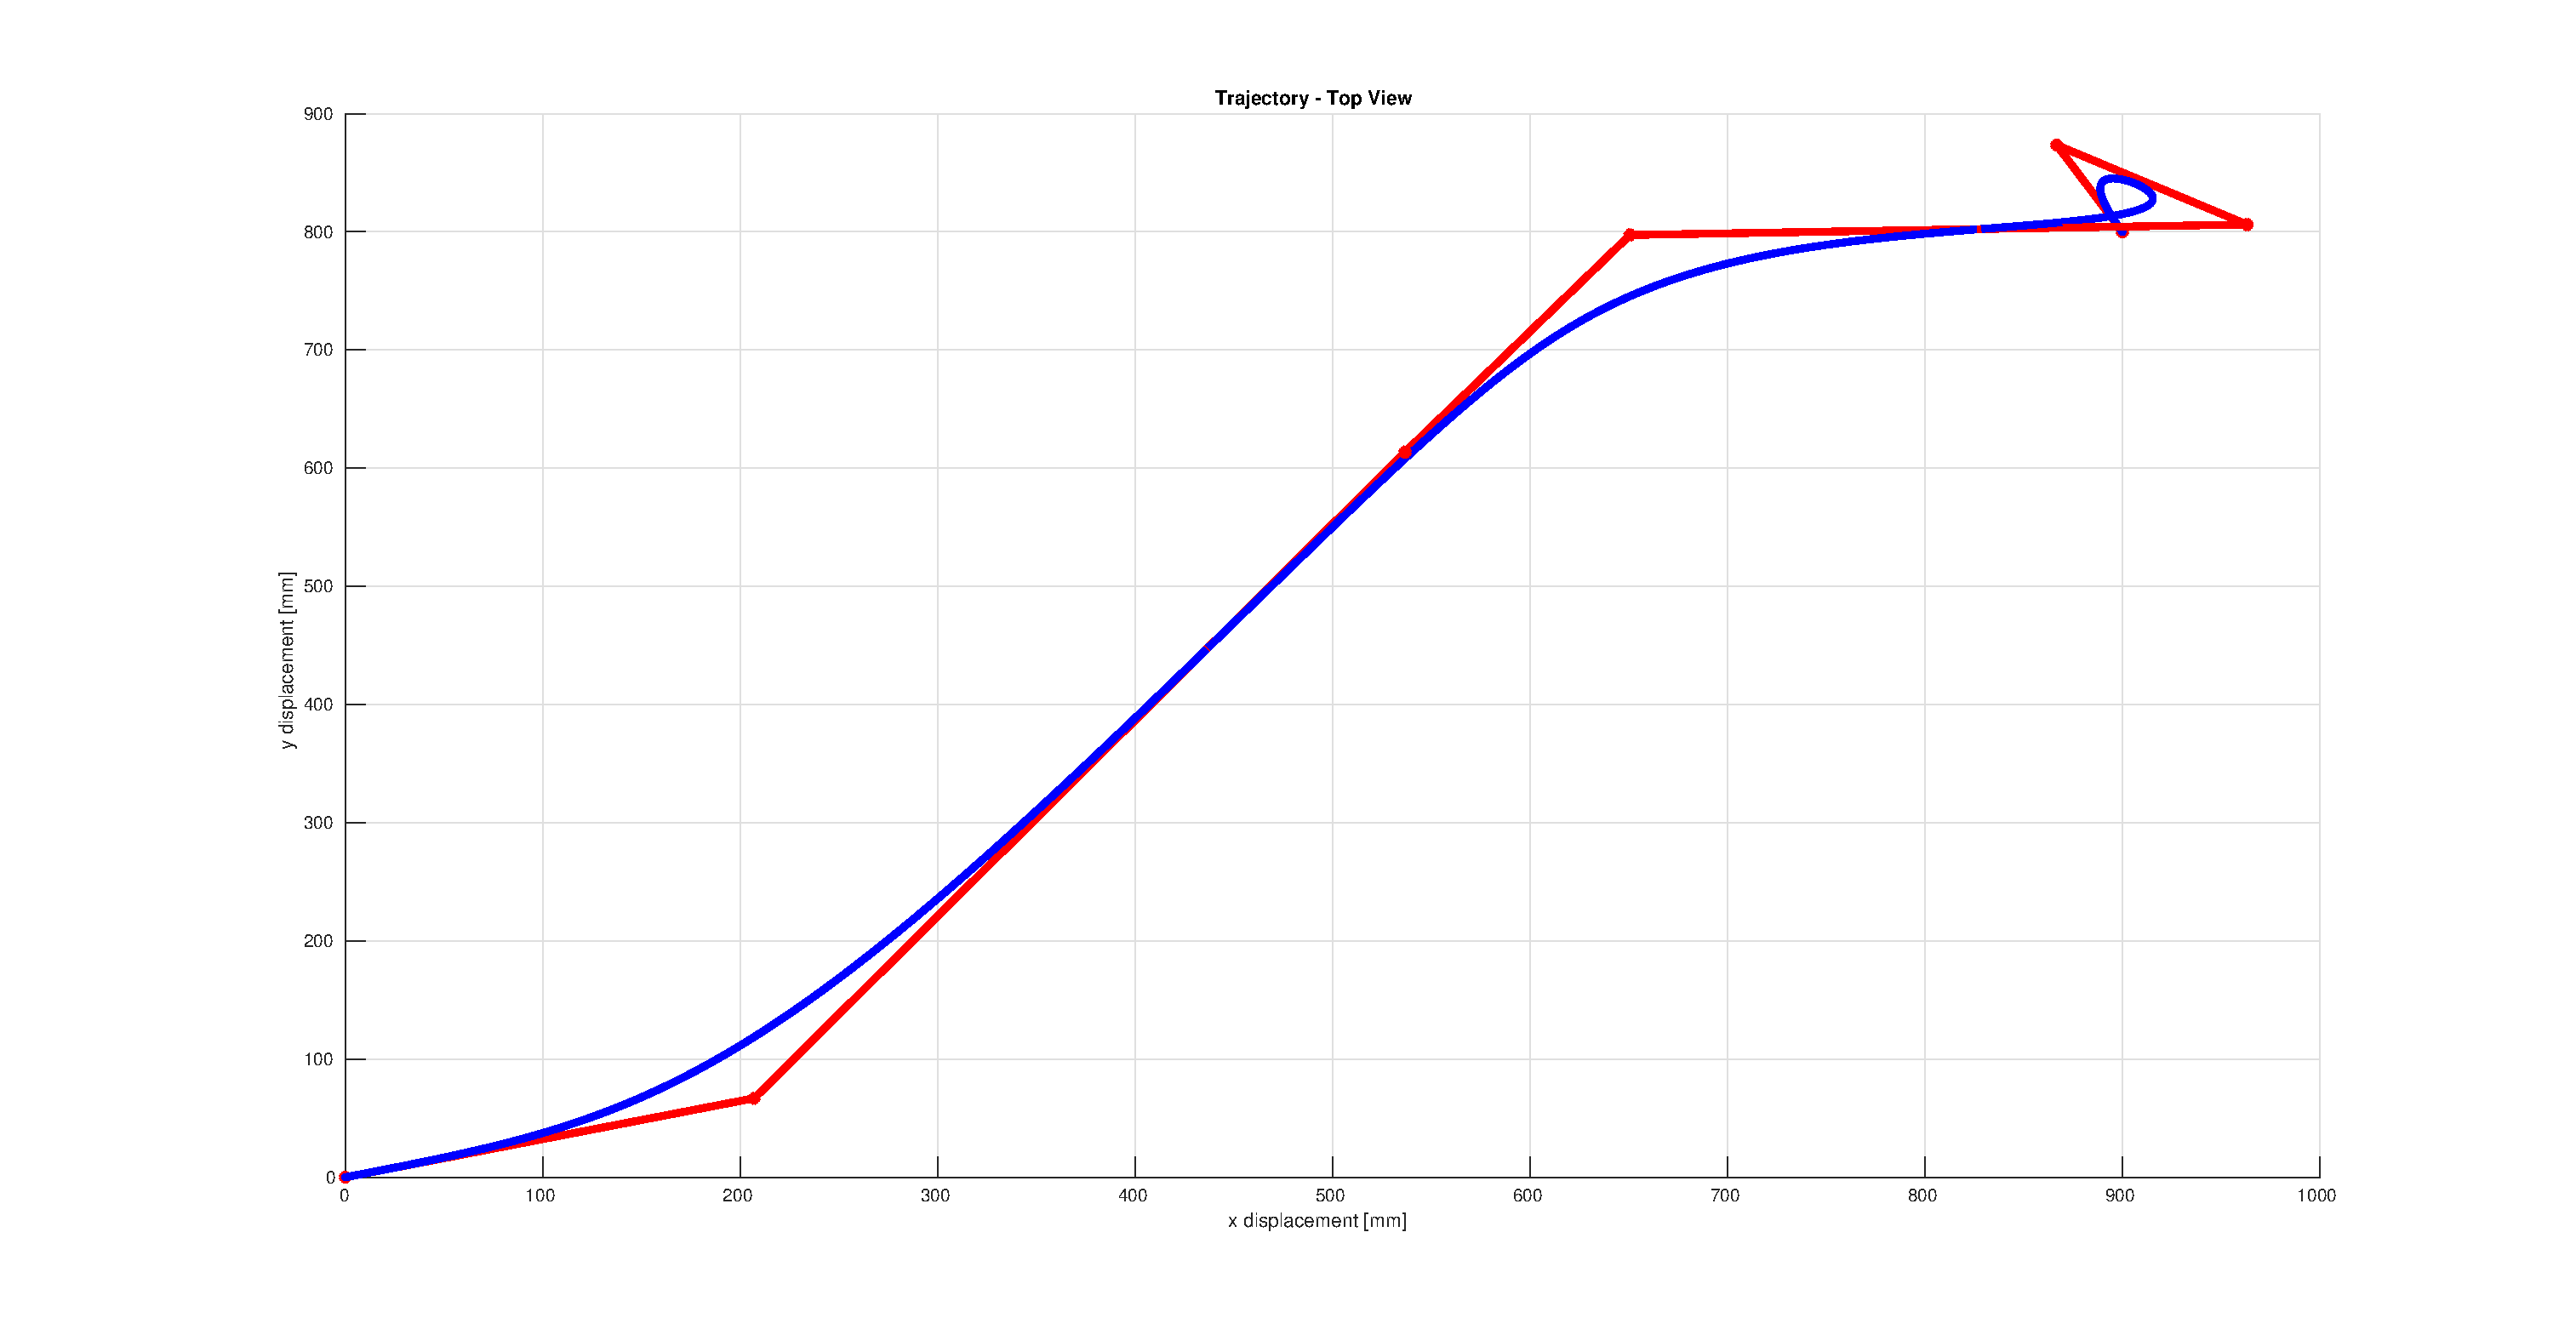
\includegraphics[height=0.45\linewidth, width=0.45\linewidth]{trajectory_simplify_subdivide_top.eps}
		\end{minipage}
		\caption{Sample Trajectory with Augmented $\setofposes$}
		\label{fig:sample_trajectory_with_augmented_set_of_poses}
	\end{figure}

	The figures show, in order, the right, front, orthogonal and top views of
	the trajectory. The red straight lines represent the path found in the
	topological graph after the path simplification algorithms of
	Section~\ref{sec:path_simplification} have been run. These lines are
	guaranteed to be free of collisions by the path-planning algorithms in
	Chapter~\ref{chap:sampling}.

	The smooth line in Figure~\ref{fig:sample_trajectory_after_simplification}
	shows what the trajectory would look like if
	Algorithm~\ref{alg:set_of_poses_augmentation} were not run. Note especially
	how, in the orthogonal view, the trajectory can be seen to completely ignore
	the corner in the front. This issue is aggravated when trajectories of a
	higher degree of smoothness are required. Higher-degree B-spline curves'
	tendency to seemingly `ignore' a control point can lead to large deviations
	from the path guaranteed in $\topologicalgraph$ and can hence lead to
	collisions.

	Figure~\ref{fig:sample_trajectory_with_augmented_set_of_poses} shows the
	effect of instead running Algorithm~\ref{alg:set_of_poses_augmentation} on
	$\setofposes$ found from $\topologicalgraph$. Note from the orthogonal view
	that the trajectory now comes much closer to the corner, yet is still able
	to keep the requested degree of smoothness. One can also note that the
	trajectory stays much closer to the control polygon. From the top and side
	views it is clear that the trajectory approximates a collection of
	rectilinear paths with smooth bends.
